\chapter{Autonomous Planar Nonlinear Systems}
\label{C:NPS}

\normalsize

In Chapter~\ref{chap:SolveOdes} we discussed how the phase line for a single
autonomous nonlinear differential equation is determined by the equilibria of 
the differential equation.  Once the equilibria and their stability properties
are known, we can find the long time or asymptotic behavior of every solution 
to a single equation, even though we do not necessarily know a closed form 
formula for that solution.  

In this chapter we discuss the corresponding and more complicated results for 
planar systems of nonlinear autonomous differential equations.  We discuss 
precisely what information about planar phase portraits is needed in order to 
be able to tell the (asymptotic) fate of all solutions.  The information that 
we need includes the equilibria and their type (as discussed in 
Chapter~\ref{Chap:PlanarQ}), periodic solutions and their stability type, and
connecting trajectories.  Once we have the needed information, we can 
determine the qualitative features of all solutions to a planar system --- 
even though we cannot write a closed form formula for these solutions.  

In Section~\ref{S:introAPNS} we experiment numerically with nonlinear planar 
systems, introducing the information that is needed to draw a qualitative 
phase plane portrait of a differential equation.  We see that we will need to 
know the equilibria and their type (saddle, sink, or source), time periodic 
solutions and their stability, and trajectories that connect these solutions 
(including stable and unstable orbits emanating from saddles).  

In Section~\ref{S:linearization} we look more closely at the role of
linearized systems of differential equations near a hyperbolic equilibrium. 
In particular, we introduce the Jacobian matrix and show numerically that 
solutions near an equilibrium behave like solutions to the linearized 
system.  Then we use the results of Chapter~\ref{Chap:PlanarQ} to understand
specific features of the local behavior of nonlinear systems near a saddle,
sink, or source in terms of the corresponding features of solutions to linear 
differential equations.

The analytic discussion of aspects of time periodic solutions is introduced 
in Section~\ref{S:periodic}.  In particular, we show how 
periodic solutions to certain systems of differential equations can be 
constructed using phase-amplitude equations in polar coordinates.

This information is then synthesized in Section~\ref{S:SPP} in terms of 
stylized phase portraits for Morse-Smale planar systems of autonomous 
differential equations.  Morse-Smale systems are differential equations with 
properties that allow us to find qualitative phase plane portraits.  
Moreover, in a sense that we will not try to make precise, most planar 
autonomous systems are Morse-Smale.  


\section{Introduction}
\label{S:introAPNS}

In Section~\ref{S:PSP&E} we discussed phase line pictures of 
a single autonomous\index{differential equation!autonomous} 
differential equation 
\index{phase!line}
\[
\frac{dx}{dt} = f(x).
\]
We saw that knowing the equilibria\index{equilibrium} and the dynamics 
near those equilibria was sufficient information for understanding 
the dynamics of all solutions.  For example, if 
\begin{equation}  \label{e:1dexample}
f(x) = x(x-1)(x-2)=x^3-3x^2+2x,
\end{equation}
then the differential equation has three equilibria located at 
$0,1$, and $2$.  From the derivative
\[
f'(x)=3x^2-6x+2
\]
we see that 
\[
f'(0)=2, \quad f'(1)=-1, \AND f'(2)=2.
\]
So the equilibria at $x=0$ and $x=2$ are unstable\index{unstable} 
(since the derivative 
is positive at these equilibria) while the equilibrium at $1$ is 
asymptotically stable (since the derivative is negative at $x=1$). 
\index{stability!asymptotic} 
Recall Theorem~\ref{T:stability1} of Chapter~\ref{chap:SolveOdes}.  
This information is summarized in the phase line picture in 
Figure~\ref{F:pp1d}.

\begin{figure}[htb]
           \centerline{%
            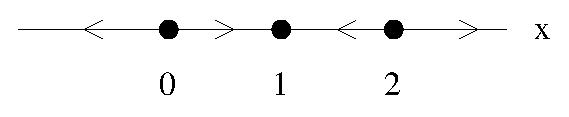
\psfig{file=figures/pp1d.eps,height=0.6in}}
           \caption{Phase line plot for the one dimensional equation
	\protect\Ref{e:1dexample}.}
           \label{F:pp1d}
\end{figure}

The added content of Figure~\ref{F:pp1d} is that we now know the 
fate of all solutions in both forward and backward time.  A 
solution $x(t)$ with initial condition at $x_0$ between the 
equilibria $0$ and $1$ approaches $1$ in forward time
($t\to\infty$) and $0$ in backward time ($t\to -\infty$).  
This information is 
encoded in the arrows on the figure.  Using {\sf dfield5}
\index{\computer!dfield5} we can 
find the time series of \Ref{e:1dexample} for an initial condition 
between $0$ and $1$.  See Figure~\ref{F:pp1dt}. Alternatively, this  
phase line tells us the equilibria and the trajectories that connect 
equilibria.  If we assume a finite number of equilibria and that the
derivative is nonzero at each equilibrium, then in one dimension 
there is nothing else that can happen in the dynamics.

\begin{figure}[htb]
           \centerline{%
            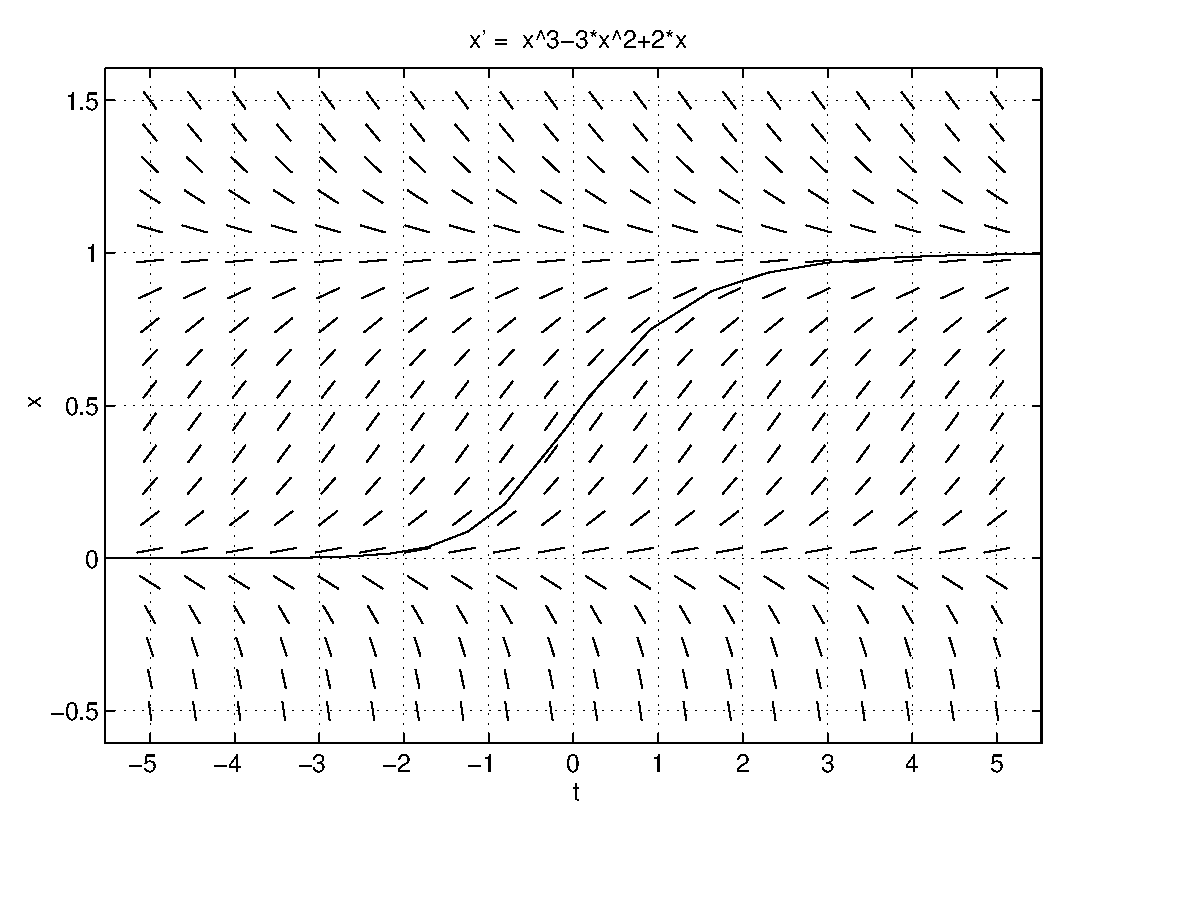
\psfig{file=figures/pp1dt.eps,height=2.0in}}
           \caption{Time series for solution to \protect\Ref{e:1dexample}
	with initial condition between $0$ and $1$.}
           \label{F:pp1dt}
\end{figure}





\subsection*{Two Dimensional Phase Planes}

The purpose of this chapter is to develop a similar understanding 
of phase portraits for two dimensional autonomous systems
\arraystart
\begin{equation} \label{e:nonlinear2}
\begin{array}{rcl} 
\dps\frac{dx}{dt} & = & f(x,y) \\
\dps\frac{dy}{dt} & = & g(x,y).
\end{array}
\end{equation}
As is the case in one dimension, equilibria and trajectories 
connecting these equilibria play a major role in determining  
phase portraits.  In two dimensions, however, there is a new 
type of solution that also plays a role in determining phase 
plane pictures: the periodic solution\index{periodic solution}.  
The remainder of this 
introduction illustrates the type of information that we will 
want to include in two dimensional phase portraits. \index{phase!plane}

\subsubsection*{A Linear Equation}

In Section~\ref{S:PlanarSystems} we saw that the dynamics of planar
constant coefficient linear differential equations are determined by the 
eigenvalues and eigenvectors of the coefficient matrix.  We  
review some of this material in Section~\ref{S:linearization}. 
For example, the origin\index{origin} is a saddle\index{saddle}
in the system of differential equations
\begin{equation*}  \label{e:localexam}
\begin{array}{rcl} 
\dps\frac{dx}{dt} & = & y \\
\dps\frac{dy}{dt} & = & 2.2x+2.1y 
\end{array}
\end{equation*}
\arrayfinish
\noindent {\bf Note:} The * after the label \Ref{e:localexam} indicates 
that this differential equation has been preloaded in the file {\tt 
e11\_1\_3.pps} and can be addressed from {\sf pplane5}
\index{\computer!pplane5} by clicking sequentially on the 
{\sf File} button in the {\sf PPLANE5 Setup} window, the 
{\sf Load a system from...} button, and the {\tt laode toolbox} button.  
Then click on the {\tt e11\_1\_3.pps} file and the {\sf Done} button to 
load the differential equation \Ref{e:localexam} into {\sf pplane5}.

The fact that the origin in \Ref{e:localexam} is a saddle is seen by 
examining the coefficient matrix of \Ref{e:localexam}
\[
C = \mattwo{0}{1}{2.2}{2.1}.
\]
Note that $\det(C)=-2.2<0$.  Since the determinant is the product 
of the eigenvalues, the eigenvalues of $C$ are real and of opposite 
sign; and the origin is a saddle.  See Table~\ref{T:hyperbolic} in 
Section~\ref{S:PlanarSystems}.

Using \Matlab we can determine more refined information
concerning the dynamics of this equation.  The two eigenvalues
of $C$ are found by entering $C$ and typing {\tt eig(C)}
to obtain
\begin{verbatim}
ans = 
   -0.7673
    2.8673
\end{verbatim}
thus verifying that the eigenvalues are real and of opposite
sign.  Moreover, we can find the eigenvectors\index{eigenvector}
\index{eigenvalue} associated with these eigenvalues by typing
\begin{verbatim}
[V,D] = eig(C)
\end{verbatim}\index{\computer!eig}
to obtain
\begin{verbatim}
V = 
   -0.7934   -0.3293
    0.6087   -0.9442
 
D =
   -0.7673         0
         0    2.8673
\end{verbatim} 
The eigenvectors are the columns of the matrix $V$ and this 
information allows us to sketch the dynamics of
\Ref{e:localexam} as in Figure~\ref{F:local} (left).  Indeed, we
can use {\sf pplane5} to plot more accurately the phase plane
picture associated to \Ref{e:localexam}, as shown in
Figure~\ref{F:local} (right).  Note also that the eigenvalue and eigenvector
information is determined in {\sf pplane5}.  In the {\sf PPLANE5 Display}
window click on the {\sf solutions} button and then on the {\sf Find an 
equilibrium} button.  Use the cross hairs to click near the origin.  Then 
{\sf pplane5} finds the equilibrium and shows the matrix $C$ and its eigenvalues
and eigenvectors in the {\sf PPLANE5 Equilibrium point data} window.

\begin{figure}[htb]
           \centerline{%
           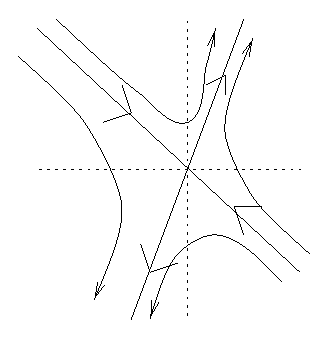
\psfig{file=figures/locala.eps,height=1.8in}
           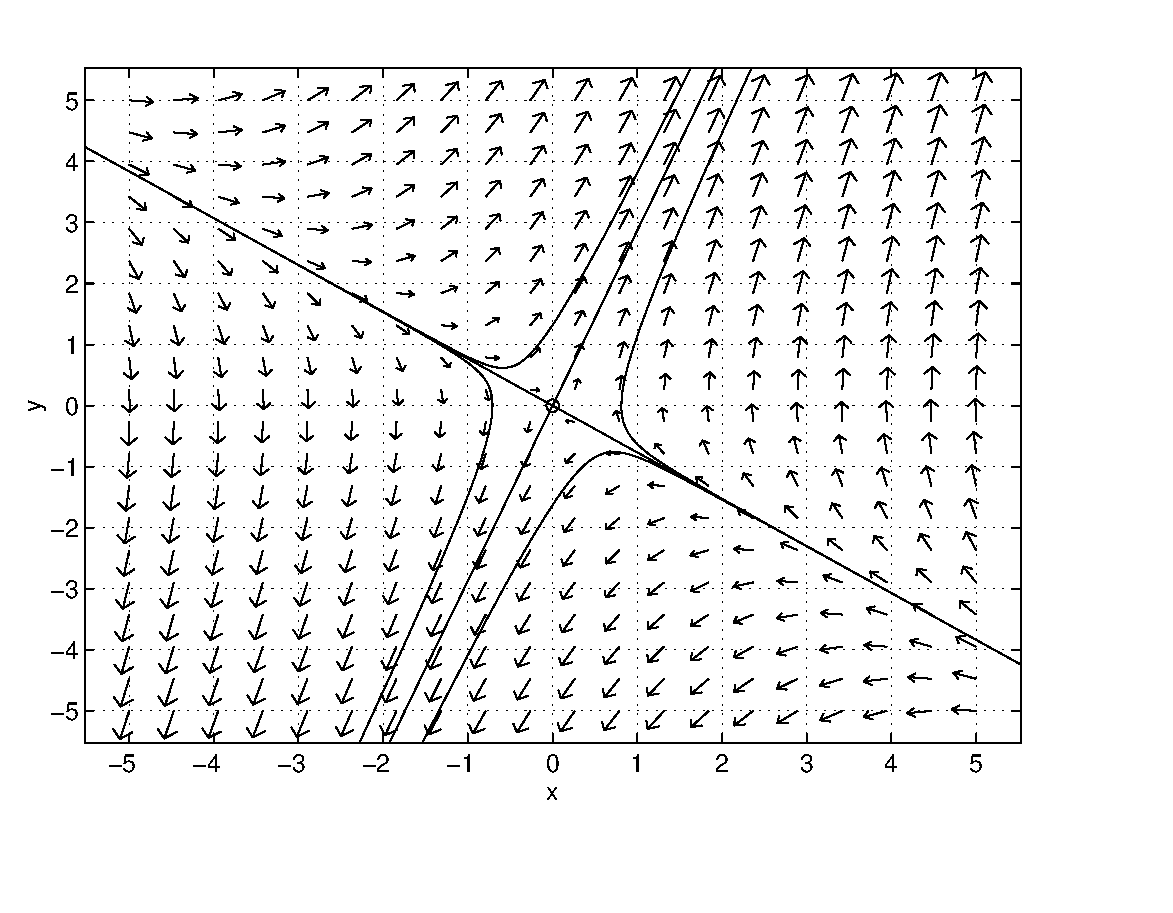
\psfig{file=figures/localb.eps,height=2.0in}}
           \caption{(Left) Sketch of phase plane of \protect\Ref{e:localexam} 
	based on eigenvalues and eigenvectors of $C$. (Right) Trajectories 
	of \protect\Ref{e:localexam} using {\sf pplane5}.}
           \label{F:local}
\end{figure}

\subsubsection*{The Addition of Nonlinear Terms}
 
Next we discuss what happens to solutions when nonlinear terms are added to 
\Ref{e:localexam}.  For example, consider the system
\index{nonlinear!system of differential equations}
\index{differential equation!nonlinear}
\arraystart
\begin{equation*}  \label{e:globalexam}
\begin{array}{rcl} 
\dps\frac{dx}{dt} & = & y \\
\dps\frac{dy}{dt} & = & 2.2x+2.1y +x^2+xy. 
\end{array}
\end{equation*}
\arrayfinish
We study the phase plane of \Ref{e:globalexam} using {\sf pplane5} and find 
that trajectories\index{trajectory} for the nonlinear system on the square 
$-0.5\leq x,y \leq 0.5$ look very much like those for the linear system 
\Ref{e:localexam} --- even though we do not know how to solve the nonlinear
system in closed form, as we can for the linear system. See 
Figure~\ref{F:globala} and note the similarity of this figure with 
Figure~\ref{F:local} (right).
\begin{figure}[hbt]
           \centerline{%
           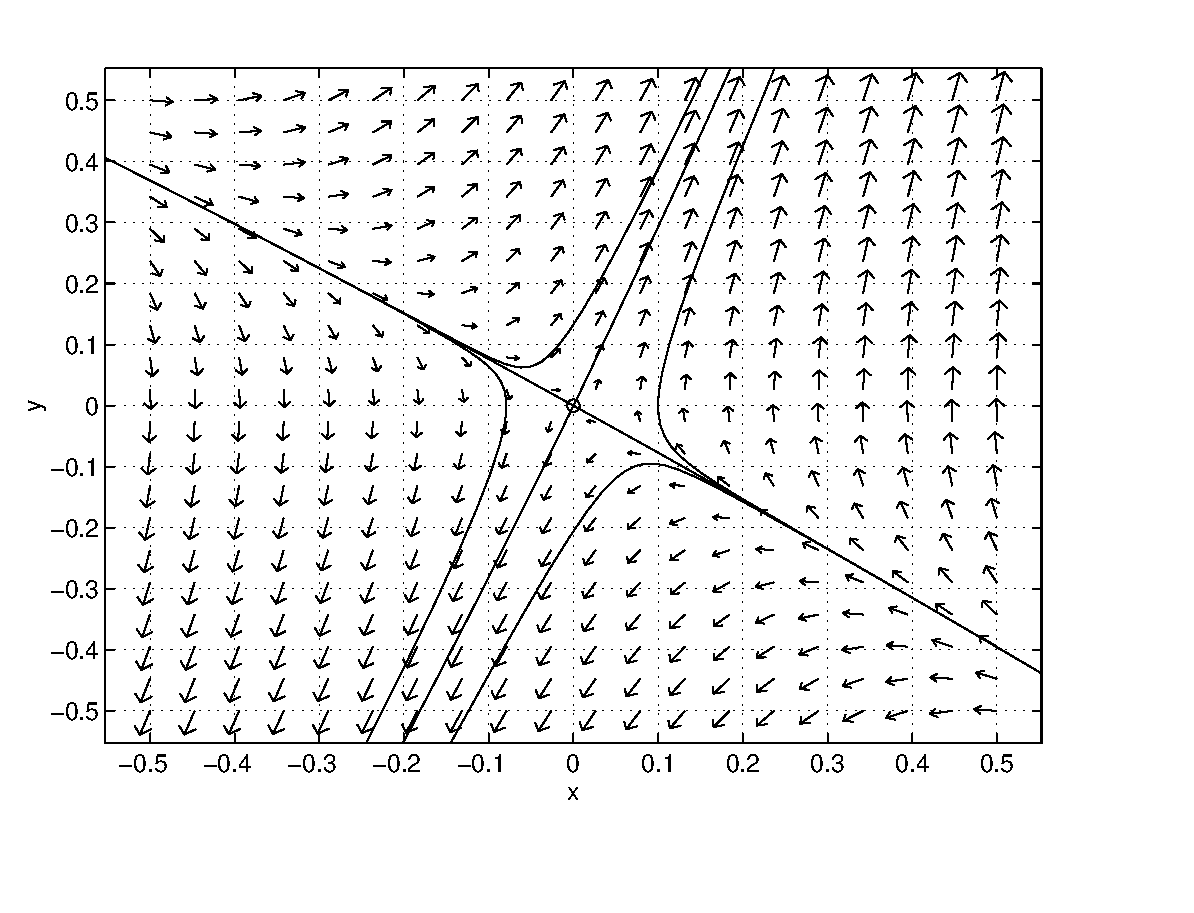
\psfig{file=figures/globala.eps,height=2.0in}}
           \caption{Trajectories of \protect\Ref{e:globalexam} 
	on the square $-0.5\leq x,y \leq 0.5$ using {\sf pplane5}.}
           \label{F:globala}
\end{figure}

Recall that an equilibrium is {\em hyperbolic\/} \index{hyperbolic} 
if the eigenvalues of
the matrix of coefficients of the linear terms have nonzero real 
part.  There is a theorem that states that in a sufficiently small
neighborhood of a hyperbolic equilibrium of a nonlinear system,
the trajectories {\em look like\/} the solutions of the
associated linear system.  Indeed, on the small square in which
these numerical calculations were performed, this theorem appears
to be correct.

However, when we compute the solution trajectories to
\Ref{e:globalexam} on the larger square $-5\leq x,y\leq 5$, it
becomes clear that the phase plane\index{phase!plane} picture of 
the nonlinear
system no longer resembles the phase plane picture of the linear
system.  See Figure~\ref{F:globalb} (left).
\begin{figure}[htb]
           \centerline{%
	   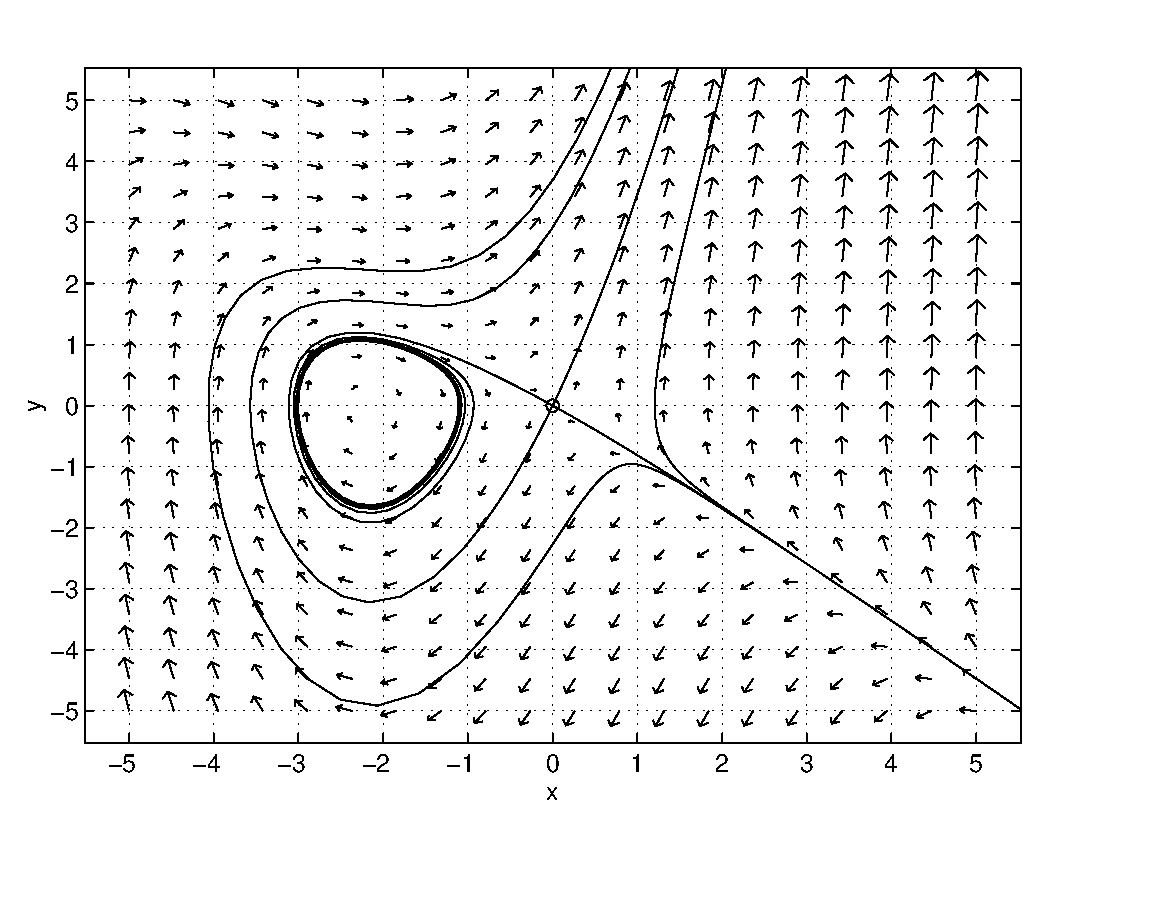
\psfig{file=figures/globalb.eps,height=2.0in}
           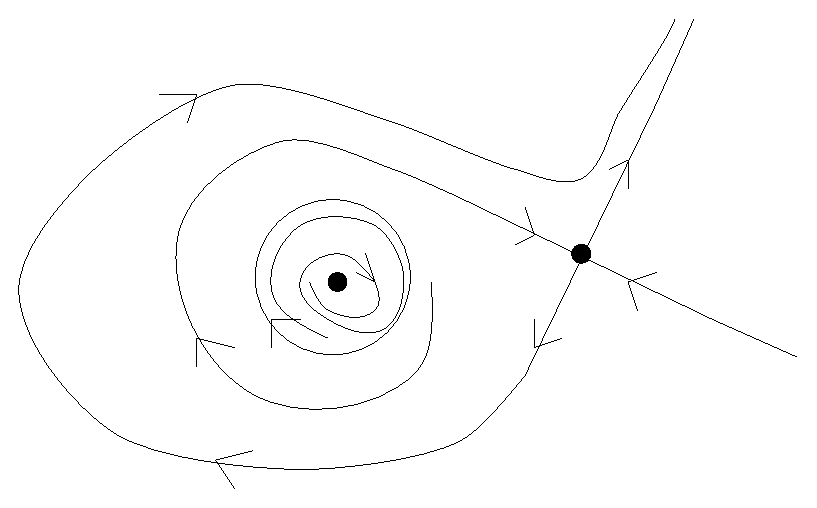
\psfig{file=figures/globalc.eps,height=2.0in}}
           \caption{(Left) Trajectories of \protect\Ref{e:globalexam} 
on the square $-5\leq x,y \leq 5$ using {\sf pplane5}. (Right) A
phase plane portrait of this equation.}
           \label{F:globalb}
\end{figure}
Note that there is another equilibrium, a spiral sink\index{sink},
surrounded by what looks like a circular trajectory.  In 
Figure~\ref{F:globalb} (right) we sketch a phase portrait for 
this system of ODEs indicating the important information: 
the equilibria and type of equilibria, the periodic solutions,
\index{periodic solution}
and the connections between these trajectories.  Note that we have found
these trajectories numerically even though we do not know how to solve for
them in closed form.

\subsubsection*{The Importance of Phase Plane Portraits}

The importance of the phase portrait is that it lets us determine the 
evolution of solutions starting in the square --- even though we do not 
have a formula for these solutions.  For example, we can use 
{\sf Keyboard input} to start a trajectory near the origin so
that its backward evolution
approaches the periodic solution
while its forward evolution leaves the square in the unstable
direction\index{unstable!direction} of the saddle\index{saddle} at 
the origin.  In Figure~\ref{F:nltraj}
we picture the trajectory in phase space through the point 
$(-0.1,0.1)$, along with the time series $y$ versus $t$ of this
solution.  

\begin{figure}[htb]
           \centerline{%
	   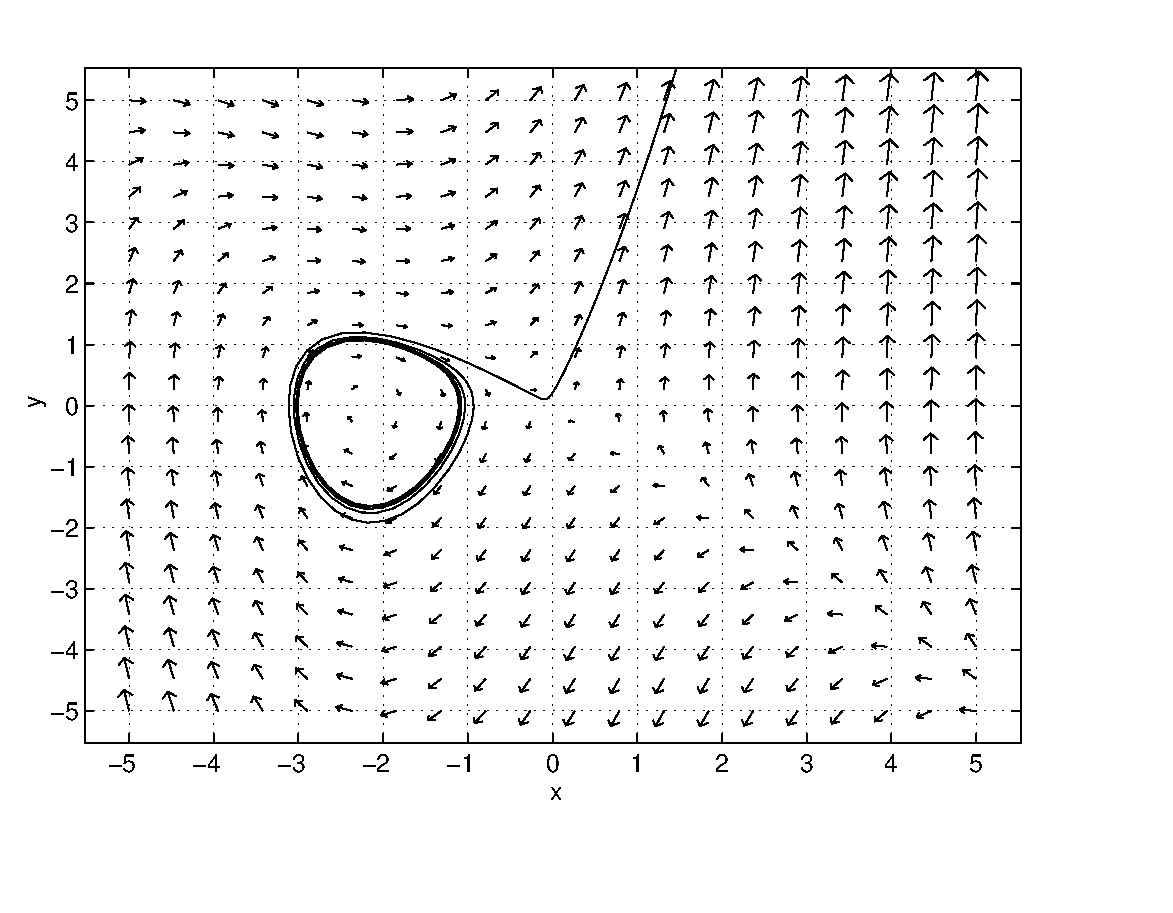
\psfig{file=figures/nltraj.eps,height=2.5in}
           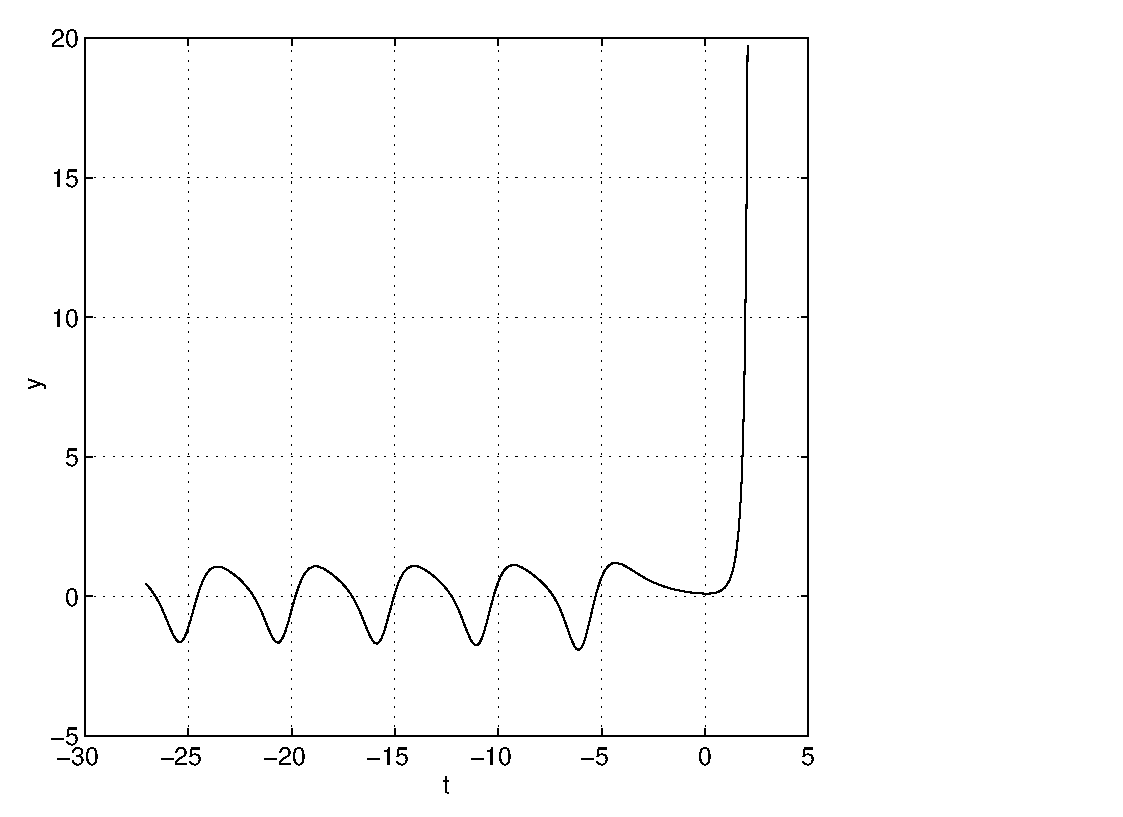
\psfig{file=figures/nlts.eps,height=2.0in}}
           \caption{(Left) Trajectory of \protect\Ref{e:globalexam} 
	through $(-0.1,0.1)$. (Right) Time series $y$ versus $t$ of
this solution.}
           \label{F:nltraj}
\end{figure}


In this chapter we discuss what kinds of dynamics we can expect
from autonomous planar systems of differential equations.  We 
show that solutions to linear systems give us much 
information about the structure of solutions to nonlinear 
systems.  We also show that there are new phenomena 
occurring in solutions to nonlinear systems that do not occur 
in solutions to the linear ones.  In our discussions we abandon 
any attempts at proofs; rather we try to survey the most 
important theorems with an eye to understanding how they can 
help with numerical explorations.

\EXER

\CEXER

\begin{exercise} \label{c8.1.1}
Use {\sf pline}\index{\computer!pline} to explore the phase line 
picture of the nonlinear differential equation
\[
\frac{dx}{dt} = 2 + 3x - 4x^2 + x^3 - 2x^4 -x^5
\]
on the interval $[-3,1]$.  Determine the number of equilibria
and whether or not they are asymptotically stable.
\end{exercise}


\begin{exercise} \label{c8.1.2}
Using {\sf pplane5}, explore the phase portraits of the nonlinear 
systems
\begin{equation*}  \label{e:global2exam}
\begin{array}{rcl}
\dot{x} & = & y \\
\dot{y} & = & 2.2x + 2.1y - x^3 + axy 
\end{array}
\end{equation*} 
where $a=1.6$ and $a=1$.  Observe that the phase planes of 
\Ref{e:global2exam} resembles the phase plane of the linear system 
\Ref{e:localexam} in the square $-0.5\leq x,y \leq 0.5$.  In the 
square $-5\leq x,y\leq 5$, discuss how these phase planes differ 
from each other and from the phase plane of \Ref{e:globalexam} 
shown in Figure~\ref{F:globalb}.
\end{exercise}

\noindent In Exercises~\ref{c8.1.3a} -- \ref{c8.1.3c} use {\sf pplane5}
to find a solution to \Ref{e:global2exam} (with $a=1.6$) satisfying the 
given properties. Plot the time series of $y$ versus $t$ for that solution 
and describe the differences in the three time series.
\begin{exercise} \label{c8.1.3a}
Find a solution that limits on the periodic solution in backwards time and 
goes to infinity in the first quadrant in forward time.
\end{exercise}
\begin{exercise} \label{c8.1.3b}
Find a solution that limits on a spiral sink in forward time and on a periodic 
solution in backwards time.
\end{exercise}
\begin{exercise} \label{c8.1.3c}
Find a solution that limits on a node in backward time and goes to infinity 
in the first quadrant in forward time.
\end{exercise}




\section{Equilibria and Linearization} \label{S:linearization}
\index{equilibrium}  \index{linearization}

Recall that equilibrium solutions of \Ref{e:nonlinear2}
are found by solving simultaneously the algebraic equations
\begin{equation}
\begin{array}{rcl} 
f(x,y) & = & 0 \\
g(x,y) & = & 0.
\end{array}
\end{equation}
In general, it is a difficult task to solve these algebraic
equations explicitly, except in the simplest of cases. One
example where an explicit solution may be found is
\Ref{e:globalexam}.  In that example, equilibria satisfy
\[
y  =  0 \AND x(2.2+x) = 0.
\]
Thus, there are two equilibria $Z_1=(0,0)$ and $Z_2=(-2.2,0)$
and these equilibria can be seen in Figure~\ref{F:globalb}.  We
know from our earlier discussion that the origin $Z_1$ is a
saddle point --- but what about the other equilibrium $Z_2$?
From the figure, it appears to be a spiral sink --- dynamics
that we associate with complex eigenvalues with negative real
parts.  See Table~\ref{T:hyperbolic} in Section~\ref{S:PlanarSystems}.  
In this section we discuss how we can apply linear theory to 
nonlinear equations. 

Let $F:\R^2\to\R^2$ be the nonlinear mapping 
\[
F(x,y)=(f(x,y),g(x,y)).
\]
\begin{Def}  \label{D:Jacobian}
The {\em Jacobian matrix} \index{matrix!Jacobian}
\index{matrix!Jacobian} of $F$ at the point 
$(x,y)$ is the $2\times 2$ matrix 
\begin{equation}  \label{e:jacobian}
(dF)_{(x,y)} = \mattwo{f_x(x,y)}{f_y(x,y)}{g_x(x,y)}{g_y(x,y)}
\end{equation}
where the subscript denotes partial differentiation.  For example, 
$f_x=\frac{\partial f}{\partial x}$.
\end{Def}

Near an equilibrium, the Jacobian matrix is the best {\em linear\/}
approximation\index{linear!approximation} to the mapping $F$.  
This statement can be formalized using 
Taylor series methods in two variables, but we just accept this fact here. 
\begin{Def}  \label{D:hyperbolic}
An equilibrium is {\em hyperbolic\/} if the eigenvalues of the 
Jacobian matrix have nonzero real part. 
\end{Def} \index{hyperbolic}\index{equilibrium!hyperbolic}

Note that it is easy to compute the Jacobian matrix for linear 
systems.  Indeed, for the linear differential equation
\begin{eqnarray*}
\dot{x} & = & ax+by \\ \dot{y} & = & cx+dy,
\end{eqnarray*}
the Jacobian matrix is just \index{matrix!Jacobian}
\[
(dF)_{(x,y)} = \mattwo{a}{b}{c}{d}
\]
and is independent of $x$ and $y$.  So, not surprisingly, the 
best linear approximation to a linear system is itself.

\begin{thm} \label{T:linearization} \index{linearization}
Suppose that the system of differential equations
\Ref{e:nonlinear2} has a hyperbolic equilibrium at
$Z_0=(x_0,y_0)$.  Then, on a sufficiently small neighborhood of
$Z_0$, the phase plane for \Ref{e:nonlinear2} is the {\em
same\/} as the phase plane\index{phase!plane} of the system of 
linear differential equations
\begin{equation}  \label{e:linearizedeqn}
\vectwo{\dot{x}}{\dot{y}} = (dF)_{Z_0} \vectwo{x}{y}.
\end{equation}
\end{thm}  \index{hyperbolic}\index{equilibrium!hyperbolic}
It is difficult to define precisely what we mean by the word
{\em same\/}. Roughly speaking, {\em same\/} means that near 
$Z_0$ there is a nonlinear change of coordinates that 
transforms the nonlinear equation into the linear one.

For example, the Jacobian matrix of \Ref{e:globalexam} at the
equilibrium $Z_2=(-2.2,0)$ is 
\[
(dF)_{Z_2} = \left.\mattwoc{0}{1}{2.2+2x+y}{2.1+x}\right|_{(x,y)=(-2.2,0)} 
= \mattwo{0}{1}{-2.2}{-0.1}.
\]
At the equilibrium $Z_2$ we may use \Matlab to show that the 
eigenvalues of $(dF)_{Z_2}$ are $-0.05\pm 1.4824i$, thus verifying 
that the equilibrium $Z_2$ is a spiral sink. \index{sink} 
It is instructive to use {\sf pplane5}\index{\computer!pplane5} to 
show the phase plane of 
the linearized system\index{linearization}.  
(To show the linearization, click on the 
{\sf Find an equilibrium point} button under the {\sf solutions} 
button.  Then in the {\sf PPLANE5 equilibrium point} window click 
on the {\sf display the linearization} button.)  The result is
shown in Figure~\ref{F:spiral} (left); compare this result 
with the phase plane picture in Figure~\ref{F:globalb} (left) 
near the spiral sink.

\begin{figure}[htb]
           \centerline{%
	   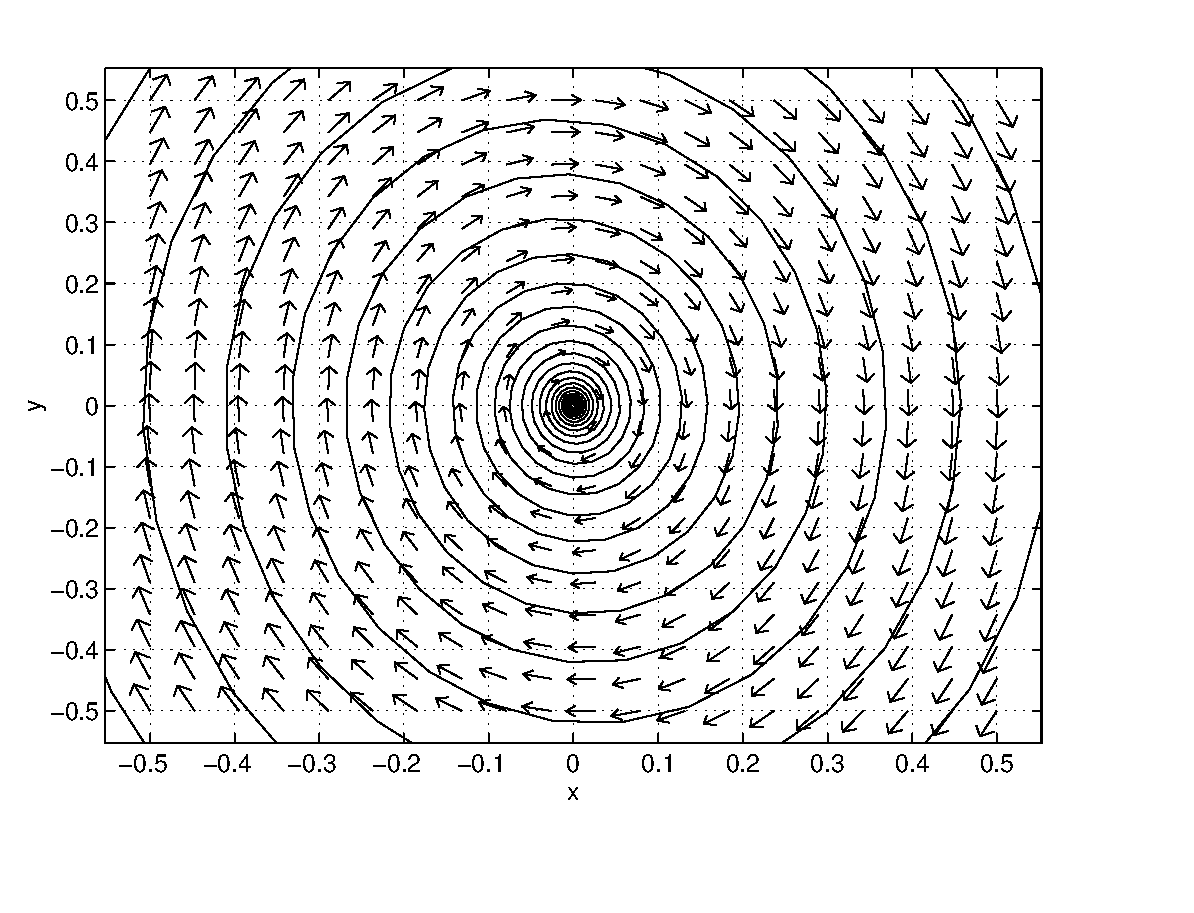
\psfig{file=figures/spirala.eps,width=3.5in}
           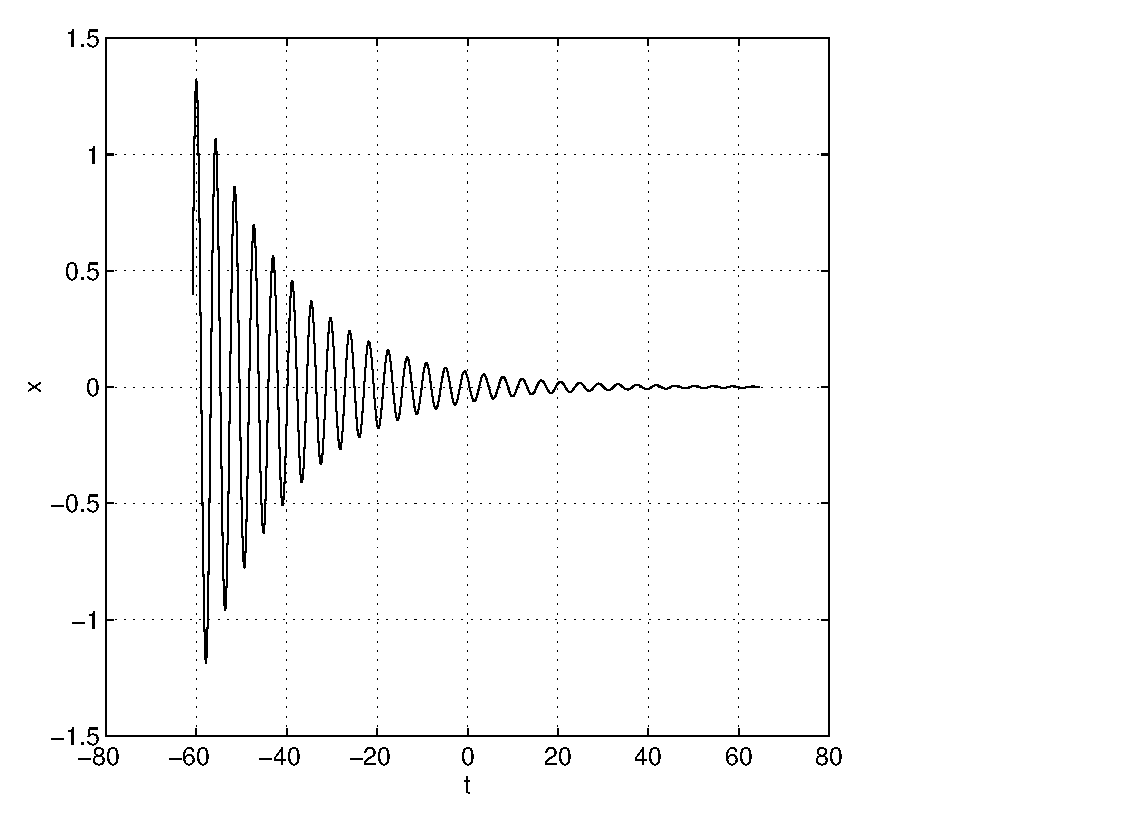
\psfig{file=figures/spiralb.eps,width=3.0in}}
           \caption{(Left) Trajectory of \protect\Ref{e:linearizedeqn} 
	     near the spiral sink $Z_2$. (Right) The time series $x$ 
		versus $t$ for this solution.}
           \label{F:spiral}
\end{figure}


There is an important corollary to Theorem~\ref{T:linearization}.
We say that an equilibrium is 
{\em linearly stable\/}\index{stability!linear}
if all of the eigenvalues of the Jacobian matrix have negative real part.

\begin{cor} \label{C:linearstability}
An equilibrium that is linearly stable is asymptotically stable.
\end{cor}  \index{stability!asymptotic} 

In Section~\ref{S:PlanarSystems} we discussed linear stability
of the origin for planar linear equations.  We showed (see
Theorem~\ref{T:linstab}) that in planar linear equations, linear
stability implies that the origin is asymptotically stable.  It
follows from Theorem~\ref{T:linearization} that the equilibrium
of the nonlinear equation is also asymptotically stable.  

\begin{rmk} 
Generalizations of Theorem~\ref{T:linearization} and 
Corollary~\ref{C:linearstability} to $n$ dimensions are both valid. 
{\rm The Jacobian matrix -- the matrix of partial 
derivatives of the coordinate functions --- is now an $n\times n$
matrix.  In $n$ dimensions, {\em hyperbolicity\/} 
of an equilibrium means that no eigenvalue of the Jacobian matrix has 
zero real part, and {\em linear stability\/} of an equilibrium means 
that the real parts of all $n$ of the eigenvalues have negative real 
part.  See Chapter~\ref{C:HDS}, Theorem~\ref{T:linstab}.}
\end{rmk} \index{hyperbolic} \index{matrix!Jacobian}

\subsection*{Important Features of Hyperbolic Equilibria}
\index{equilibrium!hyperbolic}

Theorem~\ref{T:linearization} states that a nonlinear autonomous
system of differential equations behaves like its linearization 
in a small neighborhood of a hyperbolic equilibrium.  To effectively
utilize this theorem, we need to know the important features of phase 
portraits for hyperbolic linear systems.  We now recall results of 
Section~\ref{S:PlanarSystems}.

\subsubsection*{Saddles}  \index{saddle}

Recall from Section~\ref{S:6.7} (see Definition~\ref{D:stablemfld})
that planar systems of linear differential equations with saddles at the 
origin have invariant lines (or eigendirections) called stable and unstable 
orbits.  One eigendirection corresponds to a negative eigenvalue and is 
the stable direction\index{stable!direction}, as solutions on that line 
tend to the origin in forward time.
The other eigendirection corresponds to a positive eigenvalue 
and is the unstable direction\index{unstable!direction}, as solutions on 
that line tend to the origin in backward time.

It follows from Theorem~\ref{T:linearization} that this structure is
approximately recreated in nonlinear systems on small neighborhoods of
saddles.  In particular, there are invariant curves for nonlinear systems 
defined near saddle equilibria.  The nonlinearities deform the invariant 
lines into invariant curves called {\em invariant manifolds\/}.  
\index{stable!manifold} \index{unstable!manifold}  These invariant manifolds 
are called {\em stable\/} and {\em unstable manifolds\/} or {\em stable\/} 
and {\em unstable orbits\/}\index{stable!orbit} \index{unstable!orbit}; 
stable orbits tend to the equilibrium in forward 
time and unstable orbits tend to the equilibrium in backward time.  See 
Figure~\ref{F:globalb} for an example. 

\subsubsection*{Sinks}   \index{sink}

In \Ref{e:globalexam} we have also seen that the spiraling behavior near a
spiral equilibrium is unaffected by higher order terms (see
Figure~\ref{F:globalb}); this remark is also a consequence of
Theorem~\ref{T:linearization}. Similarly, Theorem~\ref{T:linearization} 
guarantees that near an improper node\index{improper node} or a 
focus\index{focus}, higher order terms do not 
affect the local phase portrait of the nonlinear system.

\subsubsection*{An Example with Analytically Solvable Equilibria}

As an example, consider the system of ODEs
\arraystart
\begin{equation*} \label{e1:exer}
\begin{array}{crcl}
(a) & \dps\frac{dx}{dt} & = & 1 + x - y^2  \\
(b) & \dps\frac{dy}{dt} & = & -1 +6y + x^2 - 5y^2 
\end{array}
\end{equation*}
\arrayfinish
We find all of the equilibria of this system of differential
equations, and their type.  (The coefficients have been chosen
so that the calculations are feasible.  Nevertheless, it is
instructive to verify the details.)

Note that $x=y^2-1$ is the solution to \Ref{e1:exer}(a), which we
may substitute into \Ref{e1:exer}(b) to obtain
\[
y^4 - 7y^2 + 6y =0.
\]
The coefficients were chosen so that this polynomial factors
into 
\[
y(y-1)(y-2)(y+3) = 0.
\]
Thus there are four equilibria\index{equilibrium} and they are:
\[
(-1,0),\; (0,1),\; (3,2),\; (8,-3).
\]

We now determine the type of each equilibrium.  To do this,
observe that the Jacobian matrix\index{matrix!Jacobian} 
is:
\[
\left(\begin{array}{cc} 1 & -2y \\ 2x & 6-10y
\end{array}\right). 
\]
Evaluating the Jacobian matrix at the four equilibria, we obtain
\[
\mattwo{1}{0}{-2}{6}, \quad \mattwo{1}{-2}{0}{-4}, \quad
\mattwo{1}{-4}{6}{-14}, \quad \mattwo{1}{6}{16}{36}.
\]
The determinant\index{determinant}, trace\index{trace}, 
discriminant\index{discriminant}, and type of each of these
matrices is shown in Table~\ref{t:exertype}.
\begin{table}[htb]
\begin{center}
\begin{tabular}{|c|c|c|c|c|}
\hline
equilibria & det (d) & trace (t) & disc (D) & type \\
\hline
$(-1,0)$ & $6$ & $7$ & $25$ & nodal source \\
\hline
$(0,1)$ & $-4$ & --- & --- & saddle \\
\hline
$(3,2)$ & $10$ & $-13$ & 129 & nodal sink \\
\hline
$(8,-3)$ & $-60$ & --- & --- & saddle\\
\hline
\end{tabular}
\caption{Types of equilibria in Example~\protect\Ref{e1:exer}.}
\label{t:exertype}
\end{center}
\end{table}\index{nodal source}\index{saddle}\index{nodal sink}

Next we use the information about equilibria contained in 
Table~\ref{t:exertype} and {\sf pplane5}
\index{\computer!pplane5} to compute numerically the 
phase portrait\index{phase!portrait} of equations \Ref{e1:exer}.  Using 
the {\sf Find the equilibrium} button, put circles around
the four equilibria.  (Remember to make the display screen large
enough --- say $-2\leq x \leq 10$ and $-4\leq y \leq 4$.) Also
let {\sf pplane5} compute the stable and unstable orbits of
the two saddles, obtaining the picture in Figure~\ref{F:ex12}.
Once this picture is drawn we have a good idea of the phase
portrait --- note, in particular, the saddle sink and saddle
source connections.


\begin{figure}[htb]
           \centerline{%
           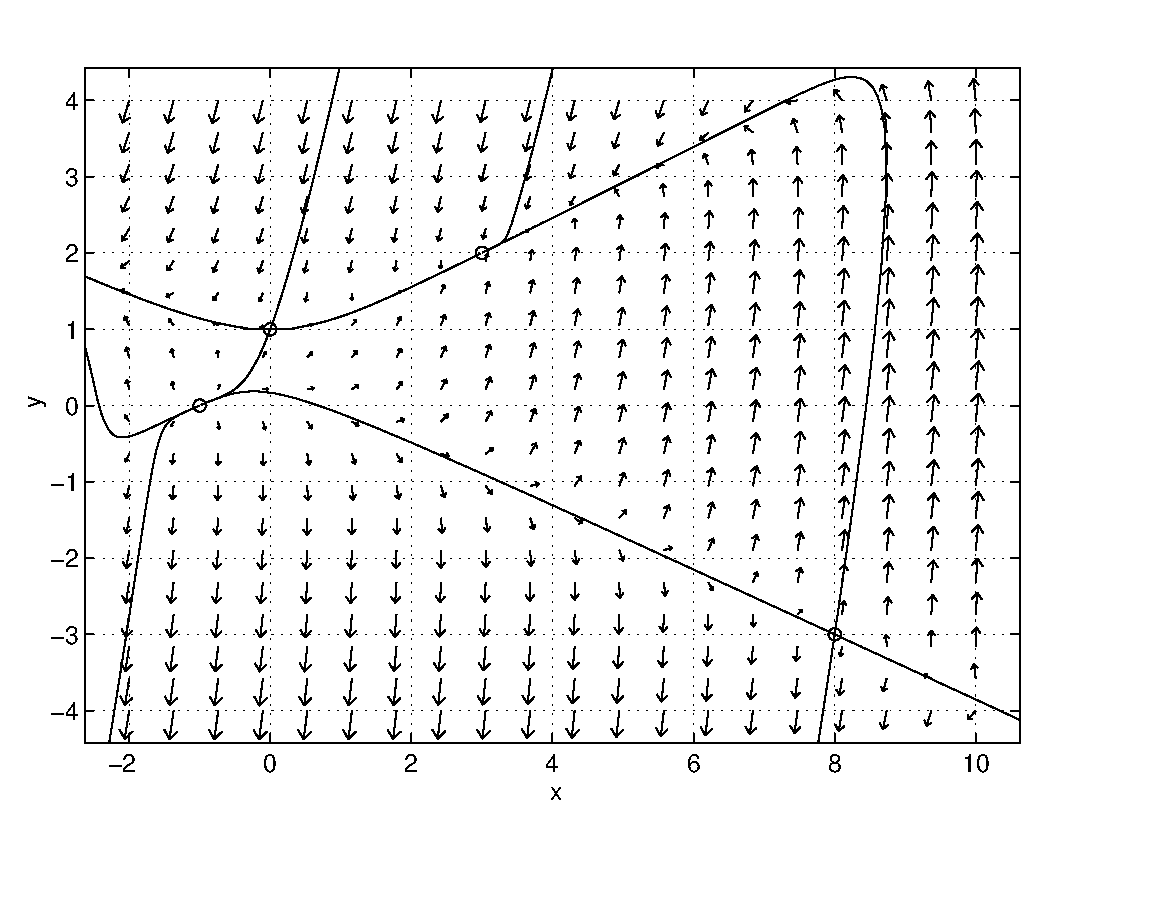
\psfig{file=figures/ex12exam.eps,width=3.5in}}
		\caption{Equilibria and connections of \protect\Ref{e1:exer}.} 
           \label{F:ex12}
\end{figure}

\subsubsection*{An Example Where Equilibria are Not Analytically Solvable}

As a second example consider the system of differential
equations
\begin{equation*} \label{e:gradexam}
\begin{array}{rcl}
\dot{x} & = & x + y + x^2 - y^2 + 0.1 \\
\dot{y} & = & y - 2xy + 0.5x^2 + y^2.
\end{array}
\end{equation*}
It is difficult to find the equilibria in \Ref{e:gradexam} explicitly.
We can, however, construct the phase plane of this equation with the 
help of {\sf pplane5}.  First we choose a square in which to display 
the direction field\index{direction field} --- say $-5\leq x,y \leq 5$. See 
Figure~\ref{F:gradexam} (left).  We then inspect the direction field 
for possible equilibria.  There is one equilibrium near the origin;  
when we use the {\sf pplane5} search feature for equilibria by clicking 
on the origin, we find a spiral source. Similarly, using the search feature 
for equilibria by clicking along the negative $x$ axis leads to a saddle.  
Once a saddle is found, instructing {\sf pplane5} to plot the stable and 
unstable orbits of this saddle helps to fill in the phase plane.  
Some experimentation yields the four equilibria and connecting stable 
and unstable orbits pictured on the right in Figure~\ref{F:gradexam}.
These equilibria, which are listed by {\sf pplane5} using the {\sf List
computed equilibrium points} button, are:
\begin{verbatim}  
(-0.1066, -0.0047)      Spiral source.           
(-1.1368, -0.2110)      Saddle point.            
(3.2539, 4.2672)        Saddle point.            
(0.2752, -0.3372)       Saddle point.       
\end{verbatim}
It is this last picture that leads to the stylized phase plane portrait 
in Figure~\ref{F:gradexamstyle}. \index{stylized phase portrait}

\begin{figure}[htb]
           \centerline{%
	   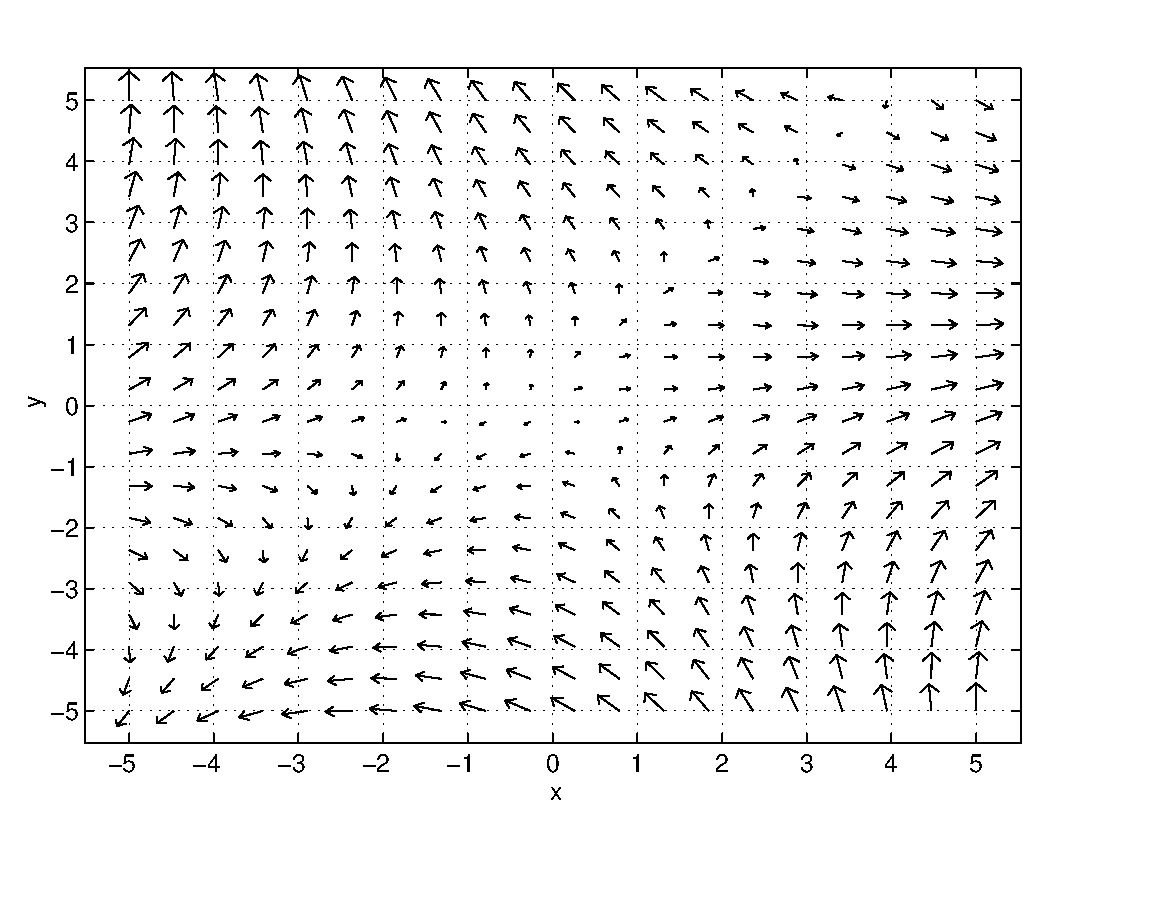
\psfig{file=figures/saddlea.eps,width=3.2in}
           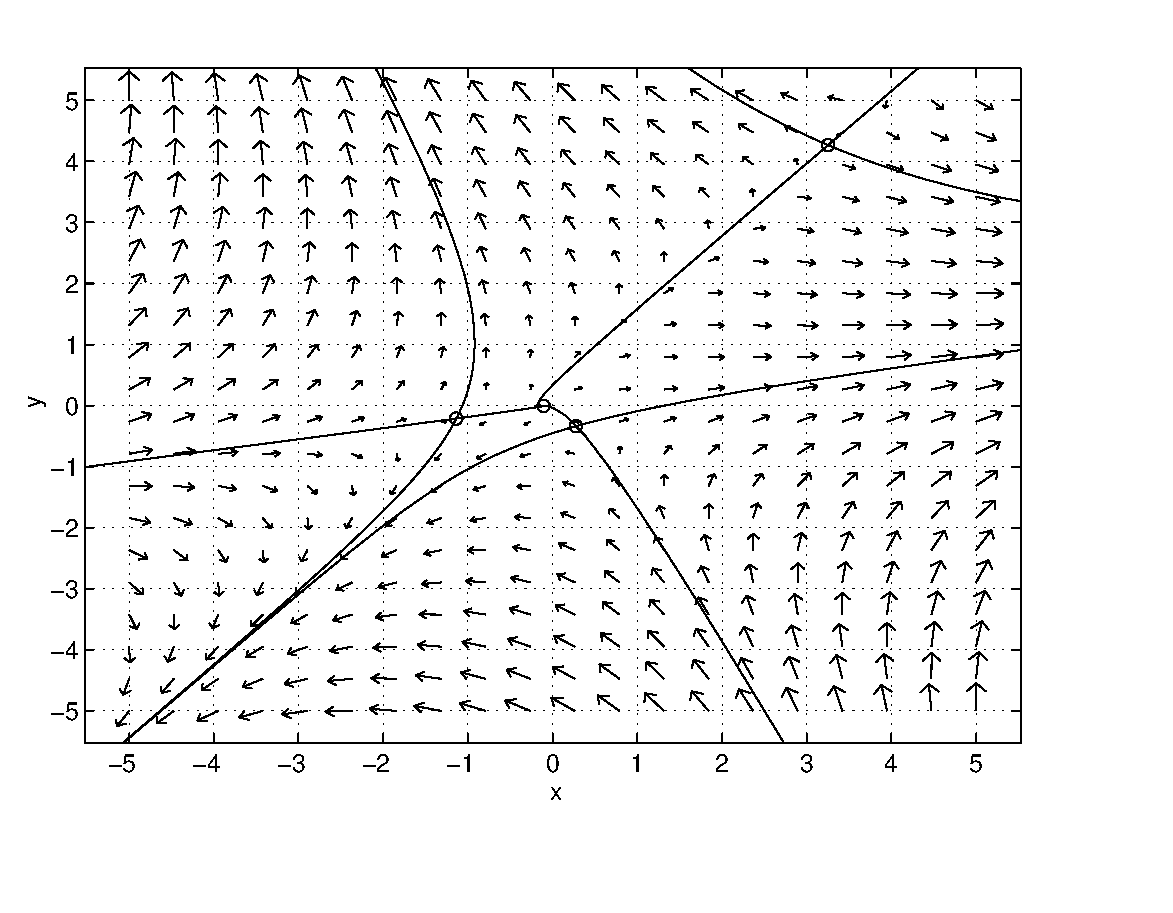
\psfig{file=figures/saddleb.eps,width=3.2in}}
           \caption{(Left) Direction field of \protect\Ref{e:gradexam}.
	(Right) Phase plane with equilibria and stable orbits.}
           \label{F:gradexam}
\end{figure}

\begin{figure}[htb]
           \centerline{%
           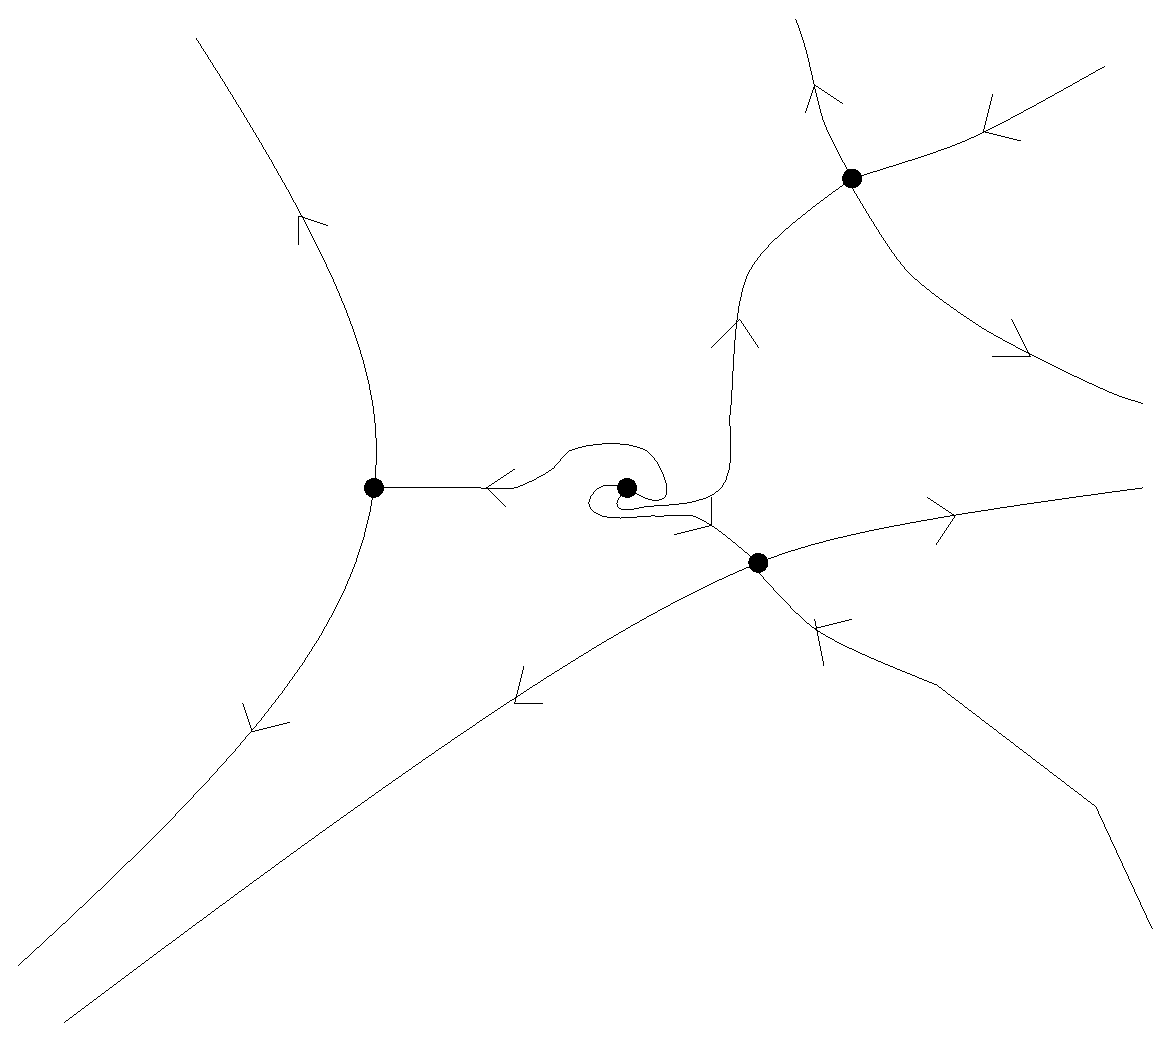
\psfig{file=figures/grad.eps,width=3.in}}
           \caption{Stylized phase plane portrait of \protect\Ref{e:gradexam}.}
           \label{F:gradexamstyle}
\end{figure}

\EXER

\TEXER

\begin{exercise} \label{c8.2.1}
\begin{enumerate}
\item[(a)] Draw the phase line picture of the differential
equation 
\begin{equation}  \label{E:quad}
\frac{dx}{dt} = -x^2 +3x -2.
\end{equation}
\item[(b)] Let $x(t)$ be the solution to \Ref{E:quad} satisfying
$x(0)=-1$.  Determine $\dps\lim_{t\to\infty} x(t)$. 
\item[(c)] Let $y(t)$ be a solution to \Ref{E:quad} satisfying
$y(0)=0.5$. Sketch the time series of this solution.
\end{enumerate}
\end{exercise}

\begin{exercise} \label{E:popex}
Recall that the simplest population growth model
\index{population model} is 
\[
\frac{dp}{dt} = \lambda p,
\]
where $p(t)$ is the population at time $t$ and $\lambda$ is the
population growth rate. Suppose that the growth rate depends on
the size of the population, as follows:
\[
\lambda(p) = \lambda_0 - ap,
\]
where $\lambda_0>0$ and $a>0$ are constants.  Suppose that
$p(t)$ is a solution and $p(0)>0$.  What is the asymptotic
limit of the population in forward time, that is, what is
$\dps\lim_{t\to\infty} p(t)$?
\end{exercise}  \index{population model}

\begin{exercise} \label{c8.2.3}
More generally, consider the population growth model
\begin{equation} \label{E:pop}
\frac{dp}{dt} = \lambda(p) p, 
\end{equation}
where the growth rate depends on the population.  Assume
\begin{enumerate}
\item[(i)] the growth rate is positive when the population is 
small, that is, $\lambda(0)>0$, and 
\item[(ii)] the growth rate decreases as the population
increases, that is, $\frac{d\lambda}{dp} < 0$ for all $p$.
\end{enumerate}
Consider the following:
\begin{enumerate}
\item[(a)] Show that equation \Ref{E:pop} has at most one
positive equilibrium $p_e>0$.
\item[(b)] Let $p(t)$ be a solution to \Ref{E:pop} with
$p(0)>0$. Determine the asymptotic limit of the population in
forward time, that is, determine $\dps\lim_{t\to\infty} p(t)$. 
\item[(c)] Relate your answer in (b) to the solution to
Exercise~\ref{E:popex}. 
\end{enumerate}
{\bf Hint:} There are two possible answers to (b) depending on
whether \Ref{E:pop} has one positive equilibrium or no positive 
equilibria.
\end{exercise}

\noindent In Exercises~\ref{c8.2.4a} -- \ref{c8.2.4e} we review some
of the theory of planar linear systems of differential equations that
is needed in the study of planar nonlinear systems.  For the given 
matrix $C$, determine whether the origin is a hyperbolic equilibrium 
for the differential equation $\dot{X}=CX$.  When the origin is 
hyperbolic, what kind of system is it?
\begin{exercise} \label{c8.2.4a}
$C=\mattwo{0.1}{2}{-1}{-3}$. 
\end{exercise}
\begin{exercise} \label{c8.2.4b}
$C=\mattwo{4}{-2}{1}{5}$. 
\end{exercise}
\begin{exercise} \label{c8.2.4c}
$C=\mattwo{2}{-1}{4}{-2}$. 
\end{exercise}
\begin{exercise} \label{c8.2.4d}
$C=\mattwo{1}{3}{-2}{-6}$.
\end{exercise}
\begin{exercise} \label{c8.2.4e}
$C=\mattwo{11}{-8}{18}{-13}$.
\end{exercise}

\begin{exercise} \label{c8.2.5}
Consider the planar nonlinear system of ODEs
\begin{eqnarray*}
\frac{dx}{dt} & = & 1 - x - y \\
\frac{dy}{dt} & = & 2xy. 
\end{eqnarray*}
\begin{itemize}
\item[(a)] Find all equilibria of this system.
\item[(b)] Determine the behavior of trajectories in a small
neighborhood of each equilibrium.
\item[(c)] Sketch the phase portrait of this system.  {\bf Hint}: Check
for invariant axes.
\item[(d)] Use {\sf pplane5} to verify your sketch.
\end{itemize}
\end{exercise}

\begin{exercise} \label{c8.2.6}
Consider the planar nonlinear system of ODEs
\begin{eqnarray*}
\frac{dx}{dt} & = & 1 - 2x + y + x^2 - xy \\
\frac{dy}{dt} & = & y - y^2
\end{eqnarray*}
\begin{itemize}
\item[(a)] Find all equilibria of this system.
\item[(b)] Are the equilibria asymptotically stable or not?
\item[(c)] Determine the type of each equilibrium.
\end{itemize}
\end{exercise}

\begin{exercise} \label{c8.2.7}
Consider the system of differential equations \Ref{e:global2exam}
that depends on the constant $a$.  
\begin{itemize}
\item[(a)]	Find the equilibria of this system.
\item[(b)]	Find the Jacobian matrices at the equilibria.  
\item[(c)]	For which values of $a$ are the equilibria not
		hyperbolic?
\item[(d)]	For those values of $a$ where the equilibria are 
		hyperbolic, determine whether or not these equilibria 
		are asymptotically stable.
\item[(e)]	For each nonhyperbolic equilibrium, write the linearized 
		system and draw its phase plane.
\end{itemize}
\end{exercise}

\begin{exercise} \label{c8.2.8}
Find all equilibria of the system of ODEs
\begin{eqnarray*}
\dot{x} & = & 2x - y \\
\dot{y} & = & 11x + x^2 - 3y^2.
\end{eqnarray*}
Also determine the types of each of these equilibria.
\end{exercise}

\begin{exercise}  \label{E:nonhyp}
\noindent (a)  Show that the origin is the only equilibrium of 
\begin{equation*}  \label{e:nonhypcenter}
\begin{array}{rcl}
\dot{x} & = & y -x^3 -2xy^2 \\
\dot{y} & = & -x - y^3
\end{array}
\end{equation*}
and that the linearized system about the origin is a 
center\index{center}. Hence the origin is not hyperbolic.

\noindent (b)  Let $r=\sqrt{x^2+y^2}$ be the distance of $(x,y)$ from the 
origin.  Let $(x(t),y(t))$ be a solution to \Ref{e:nonhypcenter} and show 
that $r(t)$ satisfies the differential equation
\[
\dot{r}(t) = -r(t)^3
\]
Use this fact to show that the origin is an asymptotically stable equilibrium
of \Ref{e:nonhypcenter}.  (Hence the phase portraits of the linearized and 
nonlinear systems are different on all neighborhoods of the origin and  
the hyperbolicity assumption in Theorem~\ref{T:linearization} is needed.)
\end{exercise}

\CEXER

\begin{exercise} \label{c8.2.10}
Use {\sf pplane5} to determine the phase portraits of the nonlinear system
\Ref{e:nonhypcenter}.  Verify that {\sf pplane5} finds (approximately) 
periodic solutions on sufficiently small neighborhoods of the origin.  This 
experiment, coupled with the results from Exercise~\ref{E:nonhyp}, suggests 
that the numerical methods employed by {\sf pplane5} fail sufficiently close 
to nonhyperbolic equilibria.
\end{exercise}

\begin{exercise} \label{c8.2.11}
Consider the system of differential equations 
\begin{equation*}
\begin{array}{rcl}
\dot{x} & = & -x - y + x^2 - y^2\\
\dot{y} & = & 0.25x - 3y - 2xy + y^2
\end{array}
\end{equation*}
\begin{itemize}
\item[(a)] Use {\sf pplane5} to verify that the origin is a nodal
sink\index{nodal sink} with 
eigenvalues $\lambda_1=-2.866$ and $\lambda_2=-1.134$.
\item[(b)] Use {\sf pplane5} on the square $-1\leq x,y \leq 1$ to 
verify that trajectories starting near the origin approach the 
origin on curves tangent to the eigendirection\index{eigendirection} 
corresponding to the eigenvalue $\lambda_2$.
\end{itemize}
\end{exercise}

\begin{exercise} \label{c8.2.12}
Using {\sf pplane5}, find all equilibria of 
\begin{equation*}
\begin{array}{rcl}
\dot{x} & = & 3x-2y-3x^2+y^2 \\
\dot{y} & = & -x+y-3xy
\end{array}
\end{equation*}
on the square $-2\leq x,y \leq 2$.  Determine the type of 
equilibria and draw a phase portrait for this system of equations. 
\end{exercise}

\section{Periodic Solutions} \label{S:periodic}
\index{periodic solution}

A periodic solution to a system of differential equations 
\begin{equation}  \label{e:genlveceqn}  
\frac{dX}{dt} = F(X)
\end{equation}
is a nonconstant solution such that 
\begin{equation}  \label{e:period}
X(t)=X(t+T)
\end{equation}
for some positive real number $T$.  The smallest positive number $T$
satisfying \Ref{e:period} is called the {\em period\/}\index{period} 
of the periodic solution.  The {\em frequency\/}\index{frequency} is 
the quantity $1/T$.
 
Uniqueness of solutions\index{uniqueness of solutions} to the initial 
value problem has an interesting consequence concerning periodic solutions.
\begin{lemma}  
Let $X(t)$ be a nonconstant solution to the autonomous
system \Ref{e:genlveceqn} such that 
\[
X(T)=X(0).
\]
Then $X(t)$ is a periodic solution with period dividing $T$.
\end{lemma}

\proof  Let $Y(t)=X(t+T)$.  Then $Y(t)$ is a solution to 
\Ref{e:genlveceqn} since 
\[
\dot{Y}(t) = \dot{X}(t+T)=F(X(t+T))=F(Y(t)).
\]
This solution has initial condition $Y(0)=X(T)=X(0)$.  
Uniqueness of solutions with the same initial condition 
implies that $X(t)=Y(t)$ for all $t$ and that $X(t)=X(t+T)$.
Since $X(t)$ is not an equilibrium, there is a smallest 
positive period for $X$ and that period must divide $T$. \qed

In this section we study two types of planar systems that have periodic 
solutions, centers and phase--amplitude equations, and in both examples 
we prove that the system has periodic solutions.  Typically, however, 
proving that periodic solutions exist is not a simple task; in general 
we rely on numerical solution to verify existence of periodic solutions..




\subsubsection*{Nonhyperbolic Centers}

Nonconstant periodic solutions occur in linear systems only when the
coefficient matrix has purely imaginary eigenvalues, that is,
when the origin is a center.  Therefore, periodic solutions
occur in linear systems only when the equilibrium is
nonhyperbolic, and they occur in infinite families.  For
example, consider the {\em center\/}  \index{center}
\begin{equation}  \label{e:planeper}
\frac{dX}{dt} = \mattwo{0}{-\tau}{\tau}{0}X.
\end{equation}
Solutions of \Ref{e:planeper} are 
\[
X(t) = \mattwo{\cos(\tau t)}{-\sin(\tau t)}{\sin(\tau t)}
{\cos(\tau t)}X_0.
\]
All nonzero solutions of \Ref{e:planeper} are periodic with period
$2\pi/\tau$.  See Figure~\ref{F:planarperiodic}.

\begin{figure}[htb]
           \centerline{%
           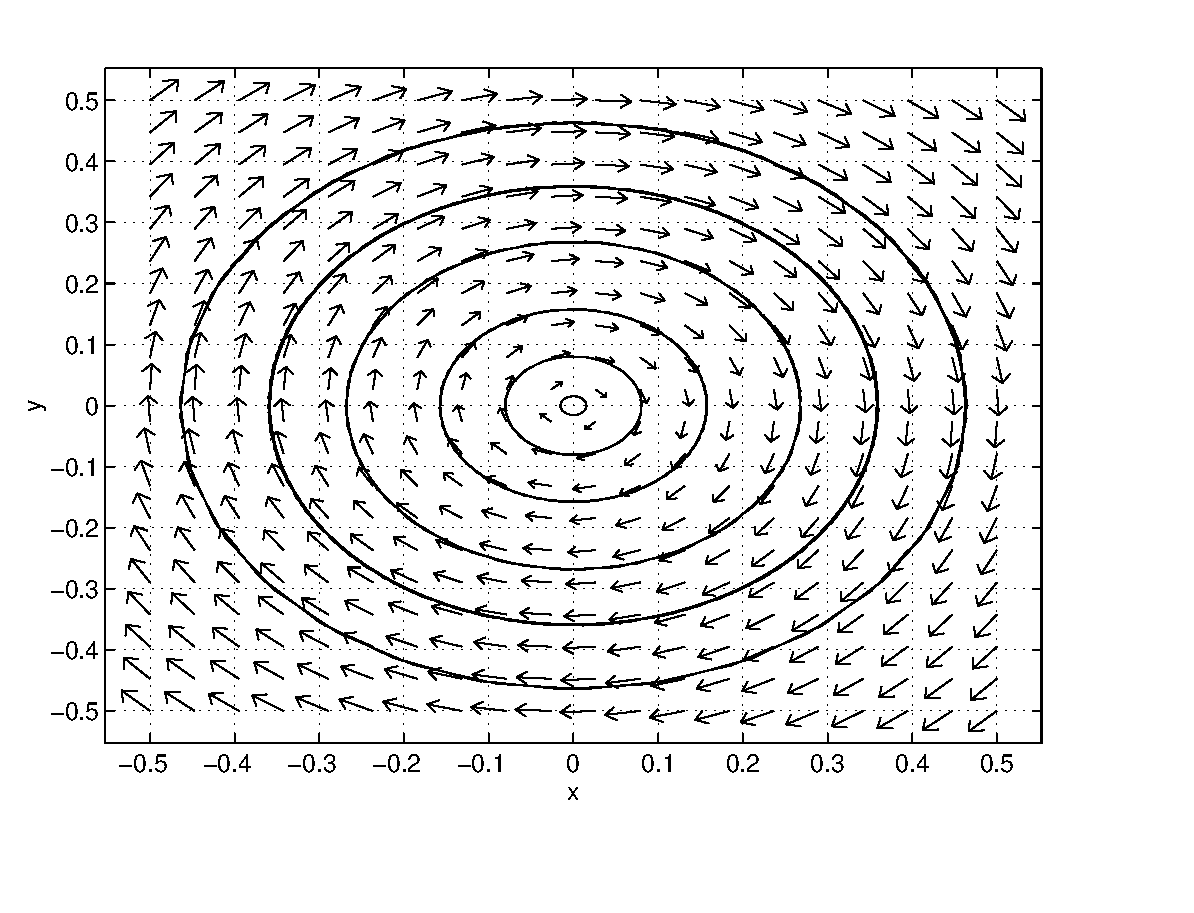
\psfig{file=figures/periodic.eps,width=3.5in}
           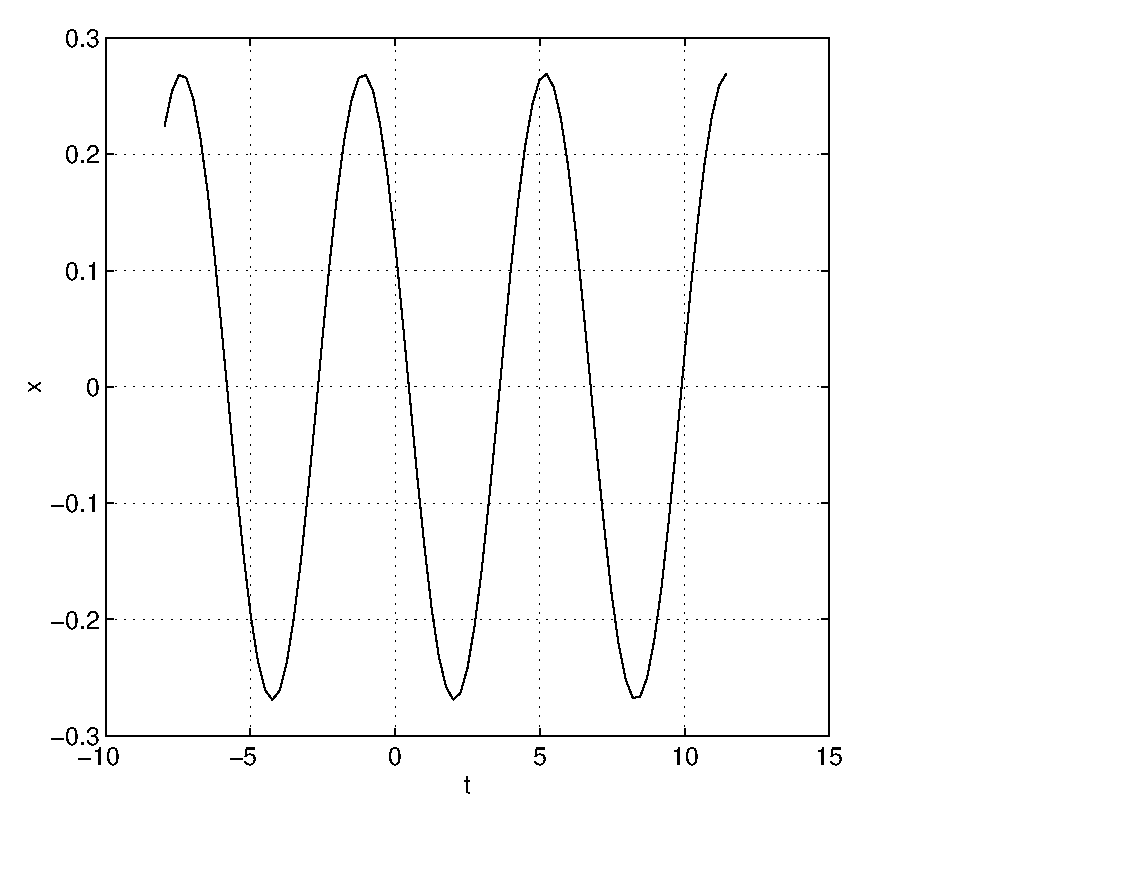
\psfig{file=figures/period2.eps,width=3.5in}}
           \caption{(Left) Trajectories of \protect\Ref{e:planeper}
	     when $\tau=3$. (Right) A time series of one solution.}
           \label{F:planarperiodic}
\end{figure}

Centers are examples of nonhyperbolic\index{nonhyperbolic}
equilibria\index{equilibrium!nonhyperbolic}, and higher
order terms will change the 
phase portrait of a center\index{phase!portrait!for a center} --- even
near the origin.  For example, consider the system  \index{hyperbolic}
\begin{equation*}  \label{e:nonlincenter}
\begin{array}{rcl}
\dot{x} & = & -2y -(x^2+y^2)x \\
\dot{y} & = & 2x - (x^2+y^2)y.
\end{array}
\end{equation*}
A trajectory in the phase portrait of \Ref{e:nonlincenter} that
spirals into the origin is shown in Figure~\ref{F:nonlincenter}
(left). Equation \Ref{e:nonlincenter} can be modified to produce
a single periodic solution, as follows:
\begin{equation*}  \label{e:nonlincenter2}
\begin{array}{rcl}
\dot{x} & = & x-2y -(x^2+y^2)x \\
\dot{y} & = & 2x+y - (x^2+y^2)y.
\end{array}
\end{equation*}
See Figure~\ref{F:nonlincenter} (right).  This example shows the necessity 
of assuming hyperbolicity as a hypothesis in Theorem~\ref{T:linearization}.  

\begin{figure}[htb]
           \centerline{%
           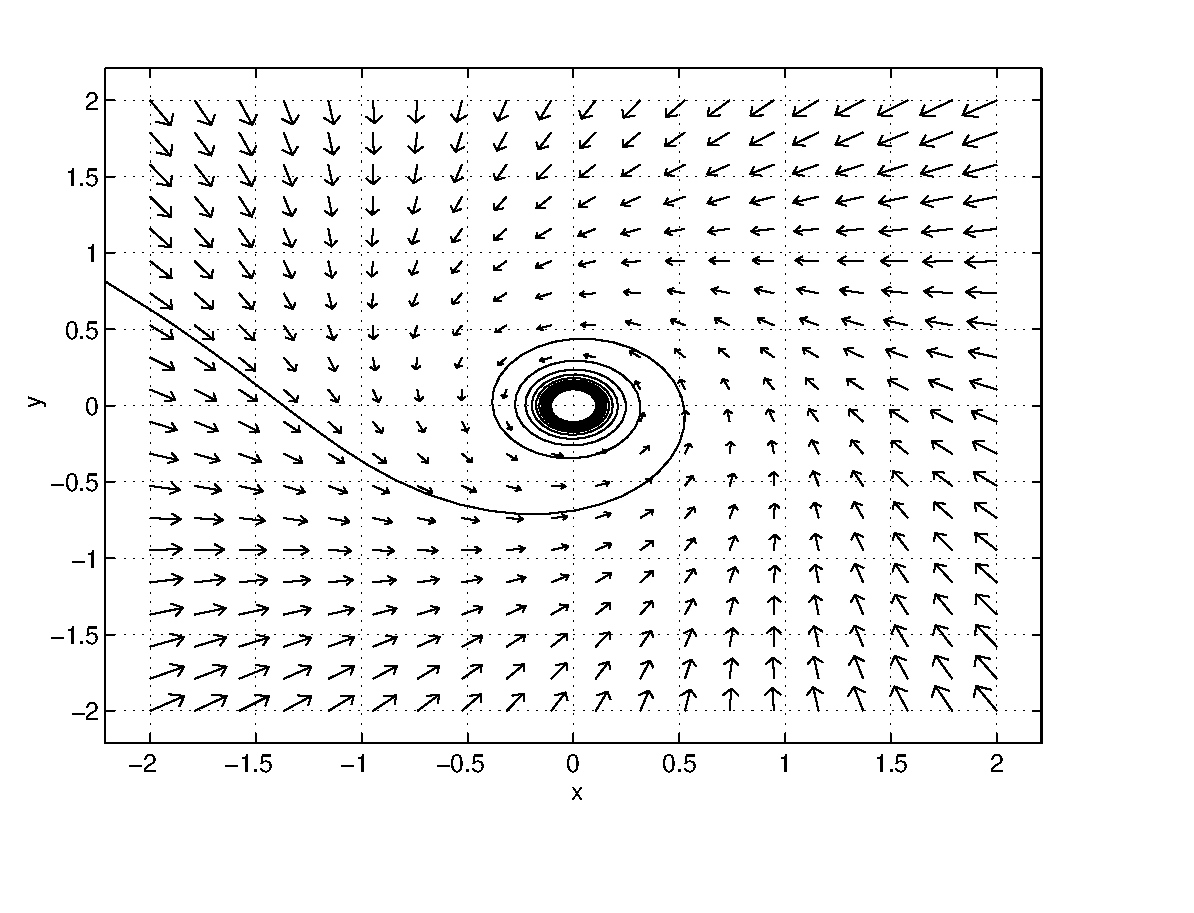
\psfig{file=figures/period3.eps,width=3.5in}
	   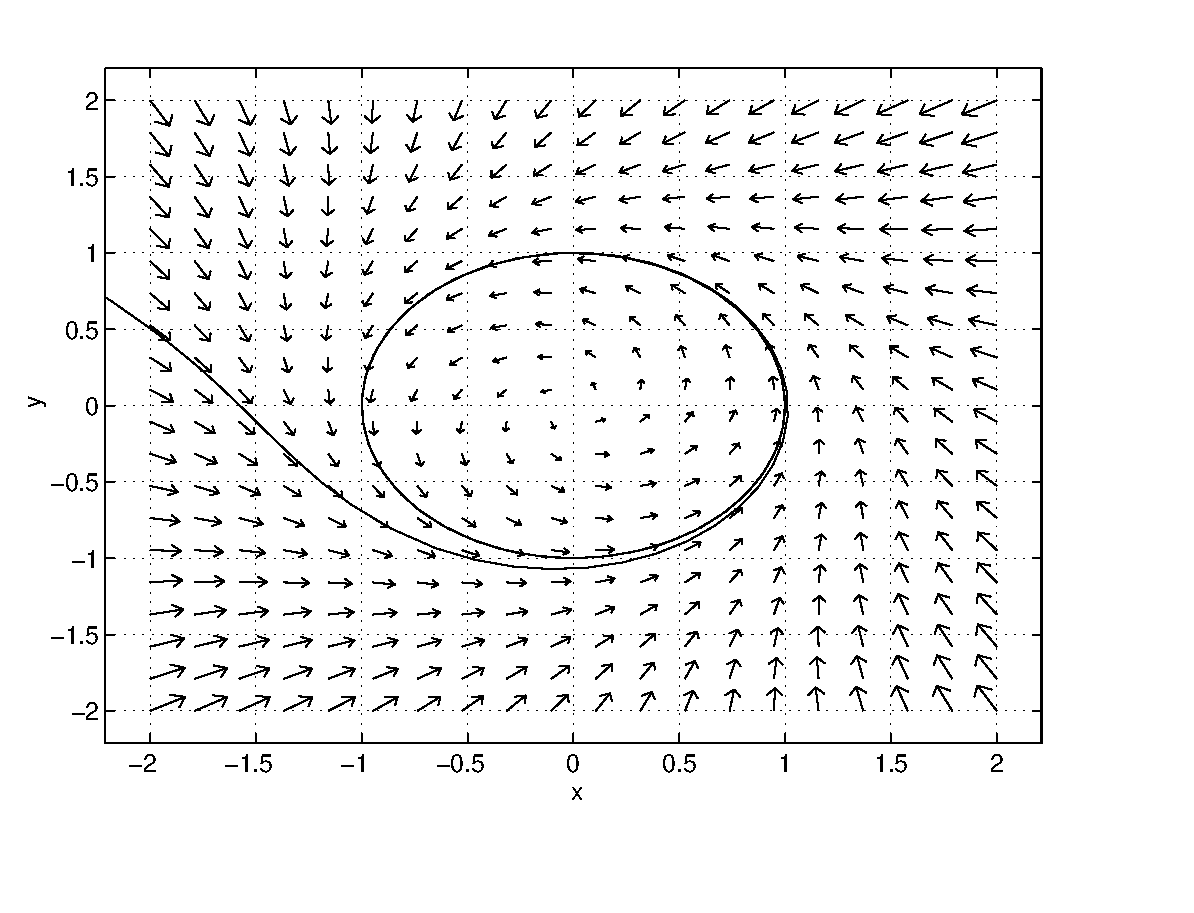
\psfig{file=figures/period4.eps,width=3.5in}}
           \caption{(Left) A trajectory of \protect\Ref{e:nonlincenter}
that spirals towards the origin. Note the slow convergence due to the fact 
that the origin is not hyperbolic.  (Right) A trajectory of 
\protect\Ref{e:nonlincenter2} that spirals towards a periodic solution.}
           \label{F:nonlincenter}
\end{figure}

\subsection*{Phase -- Amplitude Equations}
\index{phase-amplitude equations}

We now show why equations \Ref{e:nonlincenter},\Ref{e:nonlincenter2} 
behave as observed in the numerical integration.  We do this using 
polar coordinates\index{polar coordinates} and phase-amplitude equations.  
Recall that rectilinear coordinates $(x,y)$ can be written in terms 
of polar coordinates $(r,\theta)$ as
\begin{eqnarray*}
x & = & r\cos\theta\\
y & = & r\sin\theta.
\end{eqnarray*}
On inverting these equations we find that
\arraystart
\begin{equation} \label{e:polarccord}
\begin{array}{lcl}
r^2 & = & x^2+y^2  \\
\theta & = & \dps\tan\inv\left(\frac{y}{x}\right). 
\end{array}
\end{equation}
\arrayfinish
In applications, $r$ is called the {\em amplitude\/}\index{amplitude} and 
$\theta$ the {\em phase\/}.\index{phase}

Suppose that $(x(t),y(t))$ is the solution to a planar system of
ODEs of the form 
\begin{equation} \label{e:HopfNF}
\begin{array}{rcl}
\dot{x} & = & a(x^2+y^2)x - b(x^2+y^2)y\\
\dot{y} & = & a(x^2+y^2)y + b(x^2+y^2)x,
\end{array}
\end{equation}
where $a$ and $b$ are differentiable functions of $x^2+y^2$.
Note that \Ref{e:nonlincenter} and \Ref{e:nonlincenter2} are special cases 
of \Ref{e:HopfNF}.  In \Ref{e:nonlincenter} $a(r^2)=-r^2$ and $b(r^2)=2$, 
while in \Ref{e:nonlincenter2} $a(r^2)=1-r^2$ and $b(r^2)=2$.

Applying the chain rule\index{chain rule} to \Ref{e:polarccord}, we obtain 
\arraystart
\begin{equation}  \label{e:polarder}
\begin{array}{rcl}
\dot{r} & = & \dps\frac{1}{r}\left(x\dot{x} + y\dot{y}\right)\\ 
\dot{\theta} & = & \dps\frac{1}{r^2}\left(x\dot{y}-y\dot{x}\right).
\end{array}
\end{equation}
\arrayfinish
Substitute the values of $\dot{x}$ and $\dot{y}$ from \Ref{e:HopfNF} into 
\Ref{e:polarder} to obtain the 
{\em amplitude\/} equation\index{amplitude!equation}
\begin{equation} \label{e:amplitude}
\frac{dr}{dt}  =  a(r^2) r
\end{equation}
and the {\em phase\/} equation\index{phase!equation}
\begin{equation} \label{e:phase}
\frac{d\theta}{dt} =  b(r^2).
\end{equation}

\begin{prop}
Suppose that $r_0$ is a positive zero of the amplitude equation, that is,
$a(r_0^2)=0$.  If $b(r_0^2)\neq 0$, then the circle $r=r_0$ is the
trajectory\index{trajectory} of a periodic solution to \Ref{e:HopfNF}.  

Moreover, if $a'(r^2_0)<0$ then the periodic solution is asymptotically 
stable; if $a'(r^2_0)>0$ then the periodic solution is unstable.
\end{prop}\index{stability!asymptotic}\index{periodic solution}

\proof  The function $r(t)$ measures how far the solution $(x(t),y(t))$ to
\Ref{e:HopfNF} is from the origin.  Thus, if $r_0$ is a positive zero of the 
amplitude equation, then the distance of the solution remains constant; that
is, the trajectory of $(x(t),y(t))$ in the plane lies on the circle $r=r_0$
(or $x^2+y^2=r^2$ in Cartesian coordinates).  The solution to the phase 
equation corresponding to this amplitude equilibrium is 
$\theta(t)=b(r_0^2)t+\theta_0$.  Therefore, if $b(r_0^2)\neq 0$, then the 
solution trajectory moves around the circle $r=r_0$ with nonzero constant 
speed.

To verify the statement on asymptotic stability, write the amplitude 
equation as 
\[
\dot{r} = a(r^2)r \equiv f(r).
\]
The point $r_0>0$ is an equilibrium for the amplitude equation if $f(r_0)=0$, 
that is, if $a(r_0^2)=0$.  That equilibrium is asymptotically stable if 
$f'(r_0)<0$.  Using the product rule and the chain rule we see that 
\[
f'(r) = a'(r^2)2r^2 +a(r^2).
\]
Therefore
\[
f'(r_0) = 2r_0^2a'(r_0^2).
\]
It follows that $f'(r_0)<0$ if and only if $a'(r_0^2)<0$.
  
If $a'(r^2_0)<0$, then the equilibrium of the amplitude equation is 
asymptotically stable and nearby trajectories to the planar periodic solution
limit on that periodic solution $r=r_0$ in forward time.  \qed 



\subsubsection*{The Two Examples}

As noted, in both equations \Ref{e:nonlincenter} and \Ref{e:nonlincenter2}
$b(r^2) = 2$.  In the first equation $a(r^2) = -r^2$, while in
the second equation $a(r^2)=1-r^2$.  In both equations, the
phase equation is
\[
\frac{d\theta}{dt} = 2,
\]
that is solved for $\theta = 2t + \theta_0$ for some initial
$\theta_0$.  Thus all solutions spin around the origin
counterclockwise at a constant speed.  In \Ref{e:nonlincenter}
the amplitude equation is
\[
\frac{dr}{dt} = -r^3,
\]
and all solutions approach $r=0$ in forward time.  Thus, the 
phase-amplitude equations together imply that all solutions 
to \Ref{e:nonlincenter} spiral into the origin, even though the 
origin in the linearized equations is a center. 

In \Ref{e:nonlincenter2} the amplitude equation is 
\[
\frac{dr}{dt} = r-r^3.
\]
In this equation all solutions with positive initial $r$ tend towards 
$r=1$, the unit circle in the $xy$-plane.  This is seen using the one
dimensional phase line: note that there is only one positive equilibrium at 
$r=1$ and that solutions diverge from $0$ and $\infty$.  Thus, the 
phase-amplitude equations\index{phase-amplitude equations} show that 
all solutions (except the origin) spiral in forward time counterclockwise 
into the unit circle (that is a periodic solution).

\subsection*{Limit Cycles}
\index{limit cycle}

In general, for nonlinear systems without special structure, 
we do not expect periodic solutions to come in continuous families.
We do expect periodic solutions to be isolated --- as in 
Figure~\ref{F:globalb} (left).  

We call a periodic solution $x(t)$ a {\em limit cycle\/} if all 
nearby trajectories converge to $x(t)$ in forward time or all nearby
solutions converge to $x(t)$ in backward time.  Note that in phase 
space a limit cycle is always isolated; in particular, a limit cycle 
cannot be included in a continuous family of periodic solutions as 
happens in \Ref{e:planeper}.

\begin{thm} \label{T:PB}
Suppose that the right hand side of a planar system of differential 
equations is defined and smooth everywhere inside a periodic solution.  
Then there is an equilibrium inside the periodic solution.
\end{thm} 
\index{periodic solution!equilibrium inside}

This theorem is a consequence of the celebrated Poincar\'e-Bendixson theorem
\index{Poincar\'e-Bendixson theorem} and simplifies the search for limit 
cycles in the plane; limit cycles must surround at least one equilibrium.  
Again, the most important information for determining the dynamics of a given 
planar differential equation is the number and type of equilibria.  Once the 
equilibria are known, more complicated features, such as periodic 
solutions and stable and unstable orbits at saddles, can be found by 
exploration.

\EXER

\TEXER

\noindent In Exercises~\ref{c8.3.1a} -- \ref{c8.3.1c} use phase -- amplitude 
equations to determine the number of limit cycles that the given system of 
differential equations has.   Then sketch the phase portrait of this 
differential equation.
\begin{exercise} \label{c8.3.1a}
\[
\begin{array}{rcl}
\dot{x} & = &  3x-5y - 4(x^2+y^2)x + (x^2+y^2)^2x\\
\dot{y} & = &  5x+3y - 4(x^2+y^2)y + (x^2+y^2)^2y
\end{array} 
\]
\end{exercise}
\begin{exercise} \label{c8.3.1b}
\[ 
\begin{array}{rcl}
\dot{x} & = &  -5x-3y + 4(x^2+y^2)x + (x^2+y^2)^2x\\
\dot{y} & = &  3x-5y + 4(x^2+y^2)y + (x^2+y^2)^2y
\end{array}
\]
\end{exercise}
\begin{exercise} \label{c8.3.1c}
\[ 
\begin{array}{rcl}
\dot{x} & = &  6x-y - 5(x^2+y^2)x - 2(x^2+y^2)y + (x^2+y^2)^2x\\
\dot{y} & = &  x+6y - 5(x^2+y^2)y + 2(x^2+y^2)x + (x^2+y^2)^2y
\end{array}
\]
\end{exercise}

\begin{exercise} \label{c8.3.4}
Use phase -- amplitude equations to find a system of differential equations 
that has exactly three limit cycles.
\end{exercise}

\begin{exercise} \label{c8.3.5}
An autonomous planar system of differential equations is a {\em gradient\/} 
\index{gradient} system if there exists a real-valued differentiable function 
$f(x,y)$ such that 
\begin{equation} \label{E:gradsys}
\begin{array}{rcl}
\dot{x} & = & f_x(x,y) \\
\dot{y} & = & f_y(x,y).
\end{array}
\end{equation}
Prove that gradient systems never have periodic solutions.  

{\bf Hint:} Proceed in four steps as follows.
\begin{itemize}
\item[(a)]  Let $(x(t),y(t))$ be a solution to \Ref{E:gradsys} and let 
$h(t)=f(x(t),y(t))$.  So $h:\R\to\R$.  Use the chain rule to show that 
$h'(t)\geq 0$.
\item[(b)]  Show that $h'(t_0) = 0$ for some $t_0$ if and only if 
$(x(t),y(t)$ is an equilibrium of  \Ref{E:gradsys}.
\item[(c)]  Show that $h$ is monotonic increasing along any nonconstant 
solution of \Ref{E:gradsys}. 
\item[(d)]  Explain why a nonconstant solution of \Ref{E:gradsys} cannot be 
periodic.
\end{itemize}
\end{exercise}



\CEXER

\begin{exercise} \label{c8.3.2}
Verify that the system of differential equations
\begin{equation*} \label{8.3.2eq} 
\begin{array}{rcl}
\dot{x} & = & x-2y -(x^2+y^2)x + 0.1x^2\\
\dot{y} & = & 2x+y - (x^2+y^2)y - 0.2(y^2-x^2)
\end{array}
\end{equation*}
has a single limit cycle.  Compare the phase portrait of this
equation with that of \Ref{e:nonlincenter2}.
\end{exercise}

\begin{exercise} \label{c8.3.3}
Verify that the system of differential equations
\begin{equation*} \label{8.3.3eq} 
\begin{array}{rcl}
\dot{x} & = & x-2y + (x^2+y^2)^2x - 4x^3\\
\dot{y} & = & 2x+y + (x^2+y^2)^2y - 7(y^2-x^2)y
\end{array}
\end{equation*}
has a single limit cycle in the square $-2.5\leq x,y \leq 2.5$.  How many 
equilibria does \Ref{8.3.3eq} have in this square?  
\end{exercise}

\section{Stylized Phase Portraits}  \label{S:SPP}
\index{stylized phase portrait}\index{phase!portrait!stylized}


In Section~\ref{S:linearization} we discussed phase portraits of systems with 
equilibria but without periodic solutions.  In Section~\ref{S:periodic} we 
discussed briefly certain planar systems having limit cycles.  In this 
section we combine the discussions on equilibria and periodic solutions; 
together these discussions allow us to give a strategy for determining 
numerically the phase portraits of a broad class of planar autonomous 
differential equations --- the Morse-Smale differential equations.
 
Planar phase portraits indicate all equilibria, periodic
solutions, and connecting trajectories.  The simplest phase
portraits are those that describe the dynamics of differential
equations satisfying the following assumptions: \index{hyperbolic}
\begin{itemize}
\item	All equilibria are hyperbolic.
\item	All periodic solutions are limit cycles.
\item	There are no trajectories connecting two saddle points.
\end{itemize}
A planar system of differential equations that satisfies these
three conditions is called a {\em Morse-Smale\/} system.  
\index{Morse-Smale system}

\begin{Def} \label{D:stylized}
A {\em stylized phase portrait\/} of a planar autonomous system
of differential equations is a picture illustrating all
equilibria and their type, all limit cycles, and all connecting
trajectories.
\end{Def}\index{stylized phase portrait}\index{phase!portrait!stylized}

Generally, it is not an easy task to draw the stylized phase
portrait of a differential equation.  However, using {\sf pplane5\/} 
we can attempt to draw the phase portrait of a
Morse-Smale system on a given rectangle in the following way.
\begin{enumerate}
\item Using both analysis and numerics, find the equilibria of
the differential equation.
\item Mark these equilibria and their type.  
\item Draw the stable and unstable orbits of saddles.  
\index{saddle!stable and unstable orbits}
\item Determine the number and stability of limit cycles.  
\end{enumerate}
Putting this information together allows us to draw planar phase
portraits.

\subsection*{The {\sf pplane5} Default Equation}

As an example, we discuss the stylized phase portrait of the 
{\sf pplane5}\index{\computer!pplane5} default equation:
\begin{equation}  \label{e:default}
\begin{array}{rcl}
\dot{x} & = & 2x-y+3(x^2-y^2)+2xy \\
\dot{y} & = & x-3y-3(x^2-y^2)+3xy
\end{array}
\end{equation} 
Our goal is to draw the stylized phase portrait of this system
of differential equations on some rectangle in the plane, and we
choose the default rectangle: $-2\leq x\leq 4$, $-4\leq y\leq 2$.

Inspection of \Ref{e:default} shows that the origin\index{origin} 
is an equilibrium.  By clicking on the {\sf Find an equilibrium point}
button, we see that the origin is a saddle.  By clicking on the
{\sf plot stable and unstable orbits} button and then clicking
on the mouse when the cross hairs are near the origin, {\sf
pplane5} plots the stable and unstable orbits of this saddle.
See Figure~\ref{F:default0}.

\begin{figure}[htb]
           \centerline{%
	   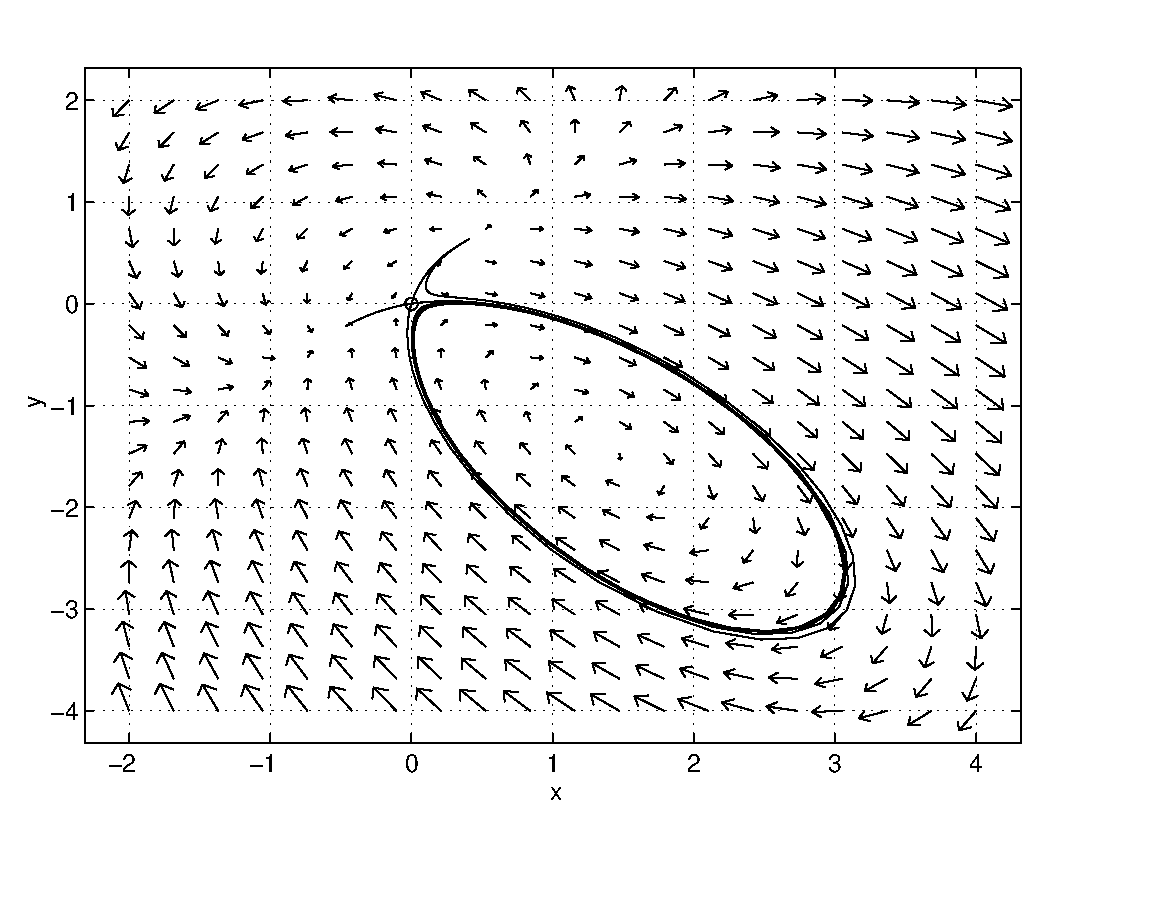
\psfig{file=figures/default0.eps,width=3.2in}
	   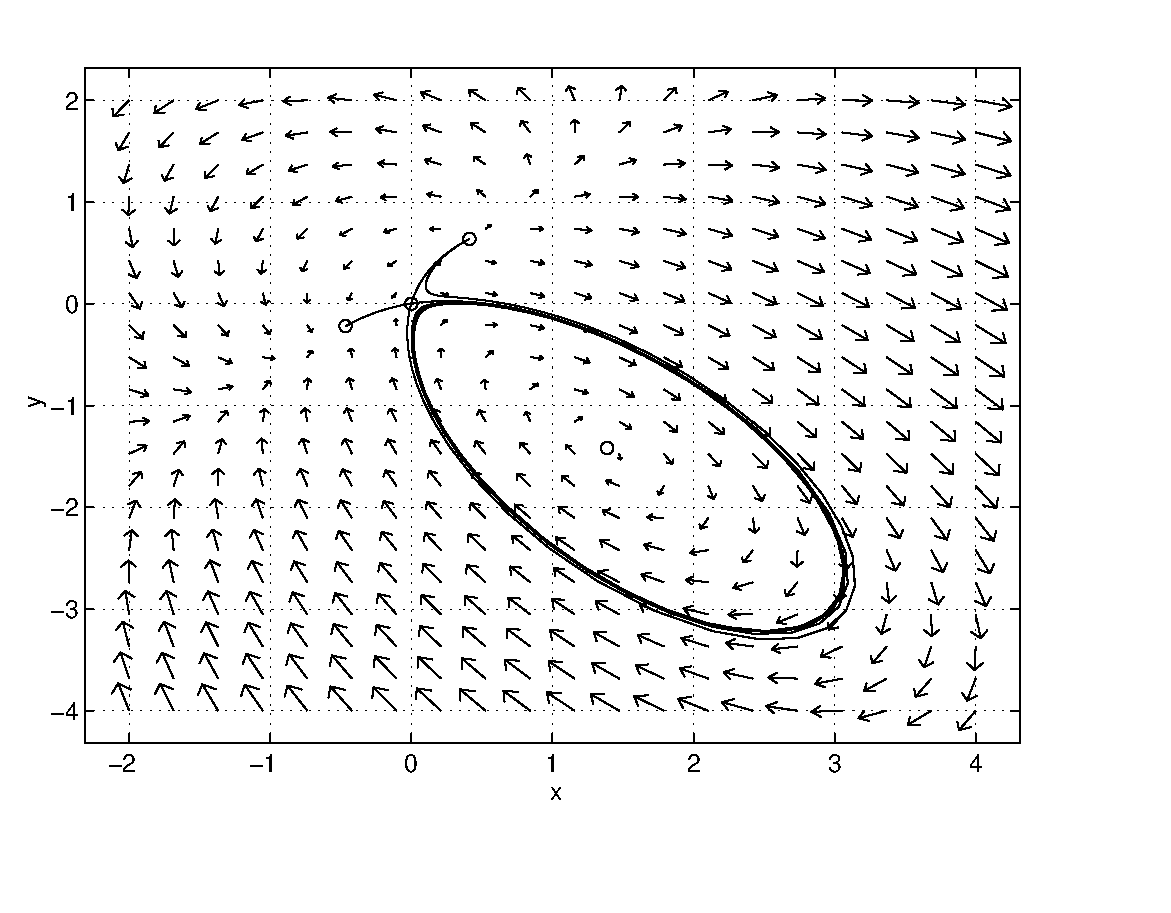
\psfig{file=figures/default1.eps,width=3.2in}}
           \caption{(Left) Stable and unstable orbits of the saddle at
		the origin in \protect\Ref{e:default}. (Right) Picture 
		of \protect\Ref{e:default} with equilibria added.}
           \label{F:default0}
\end{figure}
 
This calculation reveals several interesting features in the
phase portrait of \Ref{e:default}.  First, both stable orbits limit on the 
same equilibrium, and that equilibrium is near $(0.5,0.5)$.  Second, one 
unstable orbit limits on an equilibrium near $(-0.5,-0.2)$, while the other 
unstable orbit limits on what appears to be a limit cycle.  It follows from 
Theorem~\ref{T:PB} that there must be an equilibrium inside this limit cycle 
--- probably near $(1.3,-1.3)$.  Using the information and the {\sf
Find an equilibrium point} button, we can locate three
equilibria:
\begin{itemize}
\item	A nodal sink at $(-0.4661,-0.2209)$,
\item	A nodal source at $(0.4125,0.6386)$,
\item	A spiral source at $(1.387,-1.418)$. 
\end{itemize}
Entering these equilibria yields the phase portrait in 
Figure~\ref{F:default0} (right). 

We now draw the stylized phase portrait\index{stylized phase portrait}
\index{phase!portrait!stylized} for \Ref{e:default},
indicating the four equilibria and their type, the periodic
solutions, and the connecting trajectories. See
Figure~\ref{F:default2} (right).  A picture with additional 
trajectories is shown on the left of that figure.

\begin{figure}[htb]
           \centerline{%
	   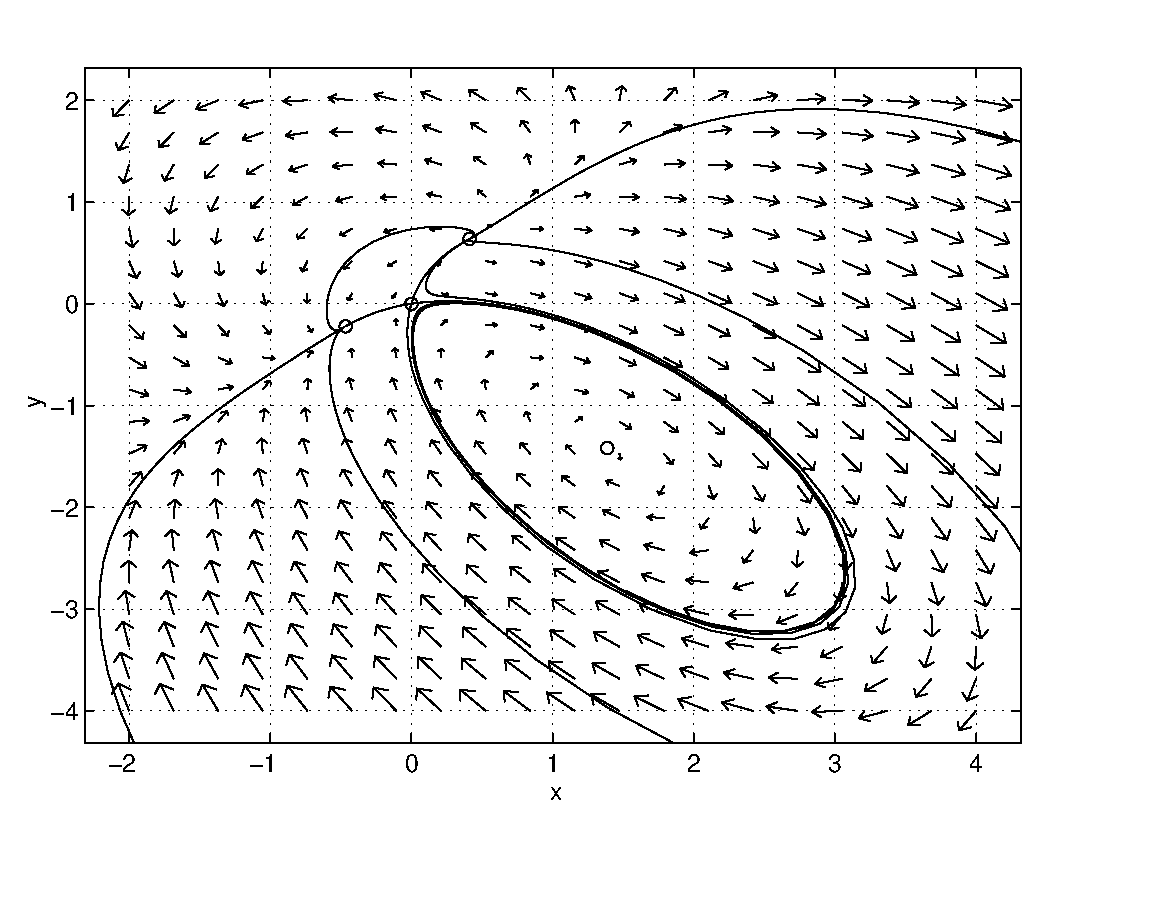
\psfig{file=figures/default2.eps,width=3.0in}
	   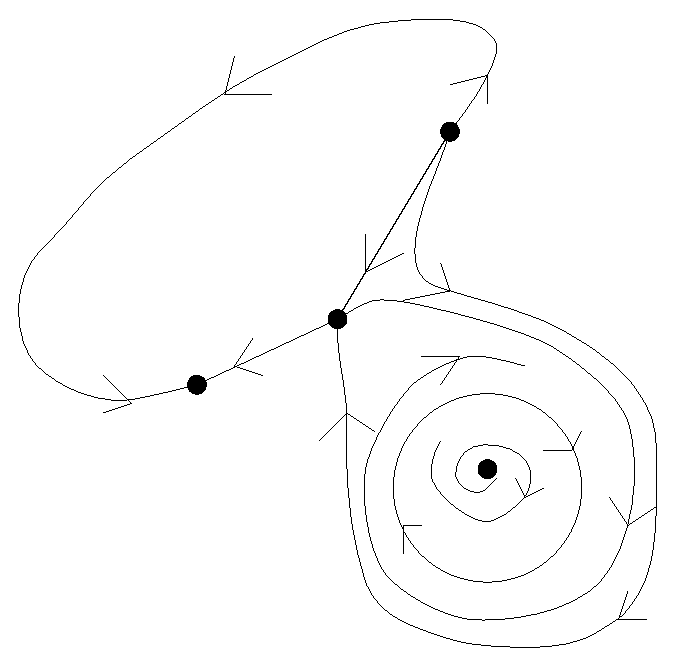
\psfig{file=figures/default4.eps,height=2.2in}
		}
           \caption{(Left) Additional trajectories of 
\protect\Ref{e:default}. (Right) Stylized phase portrait
indicating equilibria, periodic solutions and connecting trajectories.}
           \label{F:default2}
\end{figure}

It is reasonable to wonder whether this somewhat ad hoc process
for finding the stylized phase portrait will always work.  The
simple answer is {\em no} --- but much progress can be made if
one proceeds cautiously.  

For example, one numerical difficulty appears in the analysis of
the default system \Ref{e:default}.  Clicking inside the limit
cycle, shows a trajectory that spirals to a limit cycle in
forward time, as expected. In backward time, however, the
trajectory spirals towards the spiral source --- but never makes
it --- and {\sf pplane5} indicates the possible existence of a
second periodic solution.  In fact, no such periodic solution
exists. This point can be clarified using the zoom feature near
the spiral source.  These numerical calculations verify that the 
default system \Ref{e:default} is Morse-Smale.

\EXER

\CEXER

\begin{exercise} \label{c8.4.1}
Use {\sf pplane5} to determine the stylized phase portrait for 
the system
\begin{equation*}
\begin{array}{rcl}
\dot{x} & = &  2x-y+3\cos(x+y)  \\
\dot{y} & = &  x -3y -2xy
\end{array}
\end{equation*}
on the square $-10 \leq x,y \leq 10$.  Indicate all equilibria
(and their types) and all periodic solutions.
\end{exercise}  

\begin{exercise} \label{c8.4.2}
Use {\sf pplane5} to determine the number of equilibria and their
types for the system
\begin{equation*}
\begin{array}{rcl}
\dot{x} & = &  2x-y+3\cos(x+y)  \\
\dot{y} & = &  x -y -2\sin(x-y)
\end{array}
\end{equation*}
in the rectangle $-2 \leq x \leq 4$, $-3 \leq y \leq 6$.  
\end{exercise}  

\begin{exercise} \label{c8.4.3}
Use {\sf pplane5} to determine the number of equilibria and their types, the
number of limit cycles, and the connecting trajectories for the system
\begin{equation*}
\begin{array}{rcl}
\dot{x} & = & 2-y^2-((x^2-2)^2+(y^2-2)^2-1)(x^2-2)-0.2x  \\
\dot{y} & = & x^2-2-((x^2-2)^2+(y^2-2)^2-1)(y^2-2)
\end{array}
\end{equation*}
in the square $-3 \leq x,y \leq 3$.   
\begin{itemize}
\item[(a)] Draw a qualitative phase portrait for this system.  
\item[(b)] Characterize all solutions to this differential equation that 
stay within the square $-3 \leq x,y \leq 3$ for all forward and backward time 
$t$.
\item[(c)] Draw the time series in $x$ versus $t$ for the trajectory whose
initial condition is $(0,0)$.
\end{itemize}
\end{exercise}  

\begin{exercise} \label{c8.4.4}
Draw the stylized phase portrait of \Ref{8.3.3eq}.
\end{exercise}

\noindent In Exercises~\ref{c8.4.5a} -- \ref{c8.4.5b} answer the following 
four questions for the given system of differential equations:
\begin{itemize}
\item[(a)]  How many equilibria does the system of differential equations 
have?  Any equilibrium that you find using {\sf pplane5} may be considered an 
actual equilibrium.  But use analysis to prove that you have found them all.
\item[(b)]  How many limit cycles does the system of differential equations 
have?  Base your answer on numerical exploration using {\sf pplane5}.
\item[(c)]  By hand (and not necessarily to scale) sketch the phase portrait.
\item[(d)]  Indicate which initial conditions have solutions that stay
bounded in forward time.
\end{itemize}
\begin{exercise}  \label{c8.4.5a}
\begin{equation*} 
\begin{array}{rcl}
\dot{x} & = & 0.04x - y - 3y^2 + 2.5xy\\
\dot{y} & = & x - 3x^2 + 2x^2y.
\end{array}
\end{equation*}
\end{exercise}
\begin{exercise}  \label{c8.4.5b}
\begin{equation*} 
\begin{array}{rcl}
\dot{x} & = & 0.05x - y - 3y^2 + 2xy \\
\dot{y} & = & x - 3x^2 + x^2y.
\end{array}
\end{equation*}
\end{exercise}

